\PassOptionsToPackage{export}{adjustbox}

\documentclass[
11pt, paper=a4,  
listof=totocnumbered, % lists are also included in table of contents
numbers=noendperiod, % Don't add a period at the end of a chapter number
bibliography=totocnumbered, % add biblography to table of contents
]{scrreprt}
%\documentclass[]{apa7}

\usepackage{amsmath}
\usepackage{bookmark}
\usepackage{chngcntr}
\counterwithout{footnote}{chapter}
\counterwithout{figure}{chapter}
\counterwithout{table}{chapter}
    
\usepackage{scrhack}

% get custom bibliography style working without prepending [brackets]
\usepackage{natbib}
\setcitestyle{aysep={}} % remove comma as delimiter 

% breaks line at hyphens (resolves formatting issues in bibliography)
\usepackage{txfonts} % Use a Times-new-roman open-source clone
\usepackage{pythonhighlight}

% if you insist on Arial... then uncomment the following
\usepackage{helvet}
\renewcommand{\familydefault}{\sfdefault}

\usepackage{csvsimple-l3}
\usepackage{booktabs}

\usepackage{listings}
\usepackage{color}

\usepackage{caption}

\usepackage{float}

\setkomafont{chapter}{\Large} 
\setkomafont{section}{\large}
\setkomafont{subsection}{\large} 

\usepackage[left=2cm,right=2cm,top=2cm,bottom=2cm]{geometry} % margins
\addtolength{\footskip}{-0.7cm} % foot larger by 0,7 cm  (Raises the page number)

\usepackage[onehalfspacing]{setspace} % line space 1,5

\setlength{\parindent}{0pt} % Indent at start of paragraphs 0pt %originally 6pt
\setlength{\parskip}{6pt}

\usepackage[utf8]{inputenc} %UTF-8 to encode many characters => for many characters, you can just input the character and avoid a macro

\usepackage[ngerman]{babel} % german hyphenations
\usepackage[T1]{fontenc} %wichtig für Trennung von Wörtern mit Umlauten
\usepackage{microtype} % align margins

\usepackage{graphicx} % import graphics
\usepackage{placeins} % places the graphics within text
\usepackage{wrapfig}
\usepackage[export]{adjustbox}

\usepackage{enumitem}
\setlistdepth{6} % Maximal fünf Ebenen erlauben

% Nummerierungsformat festlegen
\setlist[enumerate,1]{label=\arabic*.}                     % 1., 2., 3., ...
\setlist[enumerate,2]{label=\arabic{enumi}.\arabic*.}      % 1.1, 1.2, ...
\setlist[enumerate,3]{label=\arabic{enumi}.\arabic{enumii}.\arabic*.} % 1.1.1, ...
\setlist[enumerate,4]{label=\arabic{enumi}.\arabic{enumii}.\arabic{enumiii}.\arabic*.} % 1.1.1.1
\setlist[enumerate,5]{label=\arabic{enumi}.\arabic{enumii}.\arabic{enumiii}.\arabic{enumiv}.\arabic*.} % 1.1.1.1.1
\setlist[enumerate,6]{label=\arabic{enumi}.\arabic{enumii}.\arabic{enumiii}.\arabic{enumiv}.\arabic{enumv}.\arabic*.} % 1.1.1.1.1.1

\usepackage{longtable} % Für sehr lange Tabellen, die evtl. umgebrochen werden müssen
\usepackage{pdflscape}
\usepackage{caption} % damit \captionof funktioniert

\usepackage{array}
\usepackage{colortbl}

\usepackage{xcolor}
% Definiere neue Farben
\definecolor{hellgelb}{RGB}{255, 255, 204}
\definecolor{hellblau}{RGB}{204, 229, 255}
\definecolor{hellrot}{RGB}{255, 204, 204}
\definecolor{hellgreen}{RGB}{204, 255, 229}
\definecolor{hellgrau}{RGB}{220, 220, 220}
\definecolor{low}{RGB}{204, 255, 229}  % Grün
\definecolor{medium}{RGB}{255, 255, 153} % Gelb
\definecolor{high}{RGB}{255, 165, 0}  % Orange
\definecolor{critical}{RGB}{255, 69, 0} % Rot

% Abbreviation's directory
% printonlyused - only if used
% withpage - the first occurrence's page number is listed too
\usepackage[withpage]{acronym}

% Einbinden von PDF Seiten
\usepackage{pdfpages}

%\usepackage[hidelinks]{hyperref} %https://tex.stackexchange.com/questions/823/remove-ugly-borders-around-clickable-cross-references-and-hyperlinks

\begin{document}

%TITELBLATT:!!!!!!!!!!!!!!!!!!!!!!!!!!!!!!!!!!!!!!!!!!!!!!!!!!!!!!!!!!!!!!!!!!!!!!!!!!!!!!!!!!!!!!!!!!!!!

\label{titlePage}
\begin{figure}[h]
\centering
\advance\leftskip--2cm

\includegraphics[width=0.50\textwidth]{01_resources/logo.pdf}
\end{figure}
\FloatBarrier

\vspace*{5mm}

\begin{Large} 
\begin{center}
Fallstudie
\end{center}
\end{Large} 

\vspace*{5mm}

\begin{Large} 
\begin{center}
Model Engineering (DLMDWME01)
\end{center}
\end{Large} 

\begin{large} 
\begin{center}
im Master Studiengang Data Science
\end{center}
\end{large}

\vspace*{15mm}

\begin{Large} 
\begin{center}
\textbf{Vorhersagemodell für den täglichen Bedarf an Bereitschaftsfahrenden beim DRK Berlin}
\end{center}
\end{Large}



\vspace*{20mm}

\begin{large} 
\begin{center}
Verfasser: Georg Grunsky
\end{center}
\end{large} 

\vspace*{-6mm}

\begin{large} 
\begin{center}
Matrikelnummer: IU14072015
\end{center}
\end{large} 

\vspace*{-6mm}

\begin{large} 
\begin{center}
Tutor: Markus Pak
\end{center}
\end{large} 

\vspace*{-6mm}

\begin{large} 
\begin{center}
Datum: \today
\end{center}
\end{large} 


\pagestyle{empty} % no page numbering on the cover



\renewcommand{\figurename}{Abb.}
\renewcommand{\tablename}{Tab.}

\pagestyle{plain}

\pagenumbering{Roman} %the intro is counted with roman numbers
\setcounter{page}{2} %starting with page 2 (page 1 is the titel)

\renewcommand{\thechapter}{\Roman{chapter}}
% --- too detailed for a seminar but otherwise useful
%\chapter{Blocking notice (optional)}

Useful if this document contains information that should prevent redistribution.
%\chapter{Acknoowledgements (optional)}

Thanks to....
\chapter{Abstract}

Der Berliner Rot Kreuz Rettungsdienst (DRK Berlin) projektiert den Einsatz eines Machine Learning Systems zur effizienten Planung eines Bereitschaftsdienstplanes für Einsatzfahrer:innen. Auf Basis einer erfolgten Use Case Analyse, stellt diese Arbeit den Projektplan vor und behandelt sowohl die Projektstruktur und -teamplanung als auch die Zeitplanung, die Kostenschätzung, die Stakeholderanalyse und das Risikomanagement des Projektes.

Für den Projektmanagement-Ansatz wird eine hybride Vorgehensweise verfolgt. Agile Methoden, wie Scrum, werden mit klassischen Elementen des V-Modell XT kombiniert. Das schafft eine klare Projektstruktur mit definierten Phasenübergängen und Planungswerkzeugen und gewährleistet gleichzeitig die Vorteile der flexiblen und iterativen Entwicklung. Das V-Modell XT wurde auf das notwendigste beschränkt um ein kleines Projektteam, einen geringen \glqq Overhead\grqq\ und eine modulare Struktur zu ermöglichen.

Mit den verwendeten Elementen des V-Modell XT wurde in manchen Bereichen zwar über die Vorgaben der Aufgabenstellung hinausgeschossen, die Dokumentation des Rahmenprozesses bietet jedoch eine hervorragende Unterstützung bei gleichzeitiger Ermutigung zur Flexibilität. Man bekommt das Gefühl, für den Projektstart \glqq bereit\grqq\ zu sein. Der, in der Aufgabenstellung verlangte, Projektstrukturplan kommt in der Dokumentation des V-Modell XT \citep{angermeier_v-modell-xt_2024} nicht vor. Leider ist auch in den vorgestellten Modellen des Studienmoduls \glqq Management von IT-Projekten\grqq\ \citep{iu_internationale_hochschule_management_2024}, das diesem Modul üblicherweise vorangeht, kein Projektstrukturplan abgebildet. Den ersten zufriedenstellenden Anhalt dazu lieferte \cite{wikipedia_projektstrukturplan_2022}. Beim Projektplan finden die Anforderungen der Aufgabenstellung sowie das V-Modell XT aber wieder zusammen. Als mögliche Ansatzpunkte wurden weiters The PM Minimalist Quick Start Guide \citep{greer_pm_2011} sowie die Lektüre von How Big Things Get Done \citep{flyvbjerg_how_2023} herangezogen, diese lieferten jedoch nicht die gehoffte Unterstützung für die Aufgabe.

Die inhaltliche Vorgabe des Projektes ist es, kosteneffizient die tägliche Anzahl des benötigten Bereitschaftspersonals vorherzusagen, gleichzeitig jedoch nie zu wenig Einsatzfahrende als Reserve vorzusehen. Das System und das Projekt bauen sich rund um diese Vorgabe auf. Die Planung sieht vor mit einem Entwicklungsteam in mehreren, teils parallelen Sprints, diese Minimalanforderung umzusetzen, sinnvoll um weitere Funktionen zu erweitern und das System, mit entsprechender Hardware und benutzerfreundlichen Frontends, in eine stabile Umgebung einzubetten, die sich gut in den IT-Betrieb des DRK Berlin integrieren lässt. Die wahrscheinlich langen Lieferzeiten der Hardwarekomponenten geben der Entwicklung einen zeitlichen Rahmen für die Umsetzung der Sprints. Inhaltlich wird dieses Projekt nicht als \glqq zeitkritisch\grqq\ eingestuft. Gegebenenfalls wirkt sich daher eine Verzögerung zwar auf die, der Kostenstelle des Projektes zugeschriebenen, Personalkosten jedoch nicht auf sonstige Aspekte und Abhängigkeiten der Umsetzung aus. Der Fokus der Entwicklung liegt, auch in der Priorisierung der Arbeitspakete, auf den, für das Machine Learning Modell relevanten Aufgaben. Das Vorhersagemodell selbst bildet das Herzstück der Aufgabe. In der Zeit- und Kostenschätzung wurde daher der Einsatz eines/r weiteren Data Scientist zwar erwogen, jedoch auch wieder verworfen. 

Anhand der exemplarisch dargestellten Risiken, ist auch ersichtlich, dass nicht nur ein potentieller Reputationsschaden für das DRK (aufgrund einer zu niedrig prognostizierten Anzahl nötiger Bereitschaftsfahrender und damit mangelnder Einsatzbereitschaft) das Projekt gefährden kann, sondern auch eine mögliche Ablehnung durch die Nutzer, die durch die Umsetzung mehr Verantwortung übernehmen müssen als in den derzeitigen Arbeitsprozessen. Dies sind u.a. zwei wesentliche Punkte, denen im Rahmen der Projektumsetzung, bei der Gestaltung des Modells und der Regelung der zukünftigen Arbeitsprozesse, unbedingt Rechnung getragen werden muss. Die zukünfigen Nutzer werden daher bereits ab Projektbeginn sowohl für das Requirements Engineering als auch für die Qualitätssicherung hinzugezogen. 




\section{Making of}

Ausgangspunkt dieser Arbeit war ein MachineLearning Szenario, das dem Modul \glqq Model Engineering\grqq\ \citep{pak_aufgabenstellung_dlmdwme01_2024} dieses Studienganges entnommen wurde. Dank der Zustimmung der zuständigen Tutoren wurde es möglich, dasselbe Thema in drei unabhängigen aber inhaltlich dennoch aneinander anschließenden Modulen zu bearbeiten. Dadurch ergab sich eine durchgängige Bearbeitung des Problemstellung durch mehrere Entstehungsphasen eines Machine Learning Systems hindurch. 

\begin{enumerate}
  \itemsep-8pt
  \item \textbf{Modul \glqq Data Science UseCase\grqq\ :} Analyse des Anwendungsfalls (ML-Canvas) bis zur Präsentation für die Freigabe durch das Präsidium.
  \item \textbf{Modul \glqq Technische Projektplanung\grqq\ :} die gegenständliche Arbeit
  \item \textbf{Modul \glqq Model Engineering\grqq\ :} Die Umsetzung des Vorhersagemodells mit bereitgestellten Trainingsdaten
\end{enumerate}

Die ganzheitliche Betrachtungsweise der Thematik ließ bereits jetzt  einen besseren Einblick in die Prozesse und Herausforderungen der Softwareprojektabwicklung mit  Machine Learning Aspekten entstehen.

Für die technische Bearbeitung der Aufgabenstellung wurden mehrere Werkzeuge verwendet. In vorangegangenen Modulen hat sich bereits die Kombination eines Git-Repositories für die LATEX-Dateien der Bearbeitung bewährt. Zusätzlich wurde probehalber das Repository auch einem Git-Projekt hinzugefügt um die Zeitschätzung des Projektes in Form von Iterations, Meilensteinen und Issues über das Git-Projekt zu gestalten. Dies erwies sich zwar als machbar, aber nicht als \glqq sauber\grqq\ , da im Repository, die tatsächlichen Issues der Portfoliophasen mit den fiktiven Issues des Projektes vermischt wurden. Eine Testversion der Software \glqq objectiF RPM\grqq\ \citep{microtool_gmbh_objectif_2024} unterstützte zwar der Entwicklung eines Verständnisses für die Herausforderungen in der Projektplanung, eine sinnvolle Herangehensweise und auch für Details der Umsetzung (wie zB Reviewmöglichkeiten für Anforderungen und \glqq Slicing\grqq\ von Use Cases), war jedoch für die tatsächliche Verwendung im Rahmen der Portfolioaufgabe zu Umfangreich und hätte den Rahmen gesprengt. Das GANTT-Diagramm wurde anschließend mit dem relativ intuitiv gehaltenem Tool \glqq YouTrack\grqq\ von JetBrains erstellt. Gerade, die Möglichkeit die Arbeitspakete hierarchisch zu strukturieren und zeitlich einfach anzupassen, machten das GANTT-Diagramm zu einem wertvollen Werkzeug, dass gute Einblicke in die Erfordernisse der Projektabwicklung bot.





\tableofcontents %table of contents

\renewcommand{\thechapter}{\Roman{chapter}}

% Abbreviations list

%\renewcommand\refname{Abbreviations} 
\chapter{Abkürzungsverzeichnis}
% The abbreviations list should contain all abbreviations that are not common-knowledge.
\begin{acronym}[RLHF] % the longest abbreviation here (for layout)
    \setlength {\itemsep}{-\parsep} % geringerer Zeilenabstand    	
    \acro{AI}{Artificial Intelligence}
    \acro{KI}{Künstliche Intelligenz}
    \acro{GPT}{Generative Pre-trained Transformer Model}
    \acro{PPO}{Proximal Policy Optimization}
    \acro{NLP}{Natural Language Processing}
    \acro{RLHF}{Reinforcement Learning from Human Feedback}
    \acro{FAQ} {Frequently Asked Questions}
\end{acronym}

% Acronyms should be made hyperreffed the first time they appear in text with
% \ac{GPT}  

\newpage

\renewcommand{\thechapter}{\arabic{chapter}} 
\setcounter{chapter}{0} %Reset chapter counter
\pagenumbering{arabic}

\chapter{Einleitung}

Im gewählten Szenario für diese Fallstudie geht es um die Herausforderung, die Planungslogik des Bereitschaftsdienstplans für den Berliner Rotkreuz-Rettungsdienst zu verbessern. Ursprünglich aus dem Modul Model Engineering stammend \citep{pak_aufgabenstellung_dlmdwme01_2024}, wurde diese Aufgabenstellung, nach Rücksprache mit den jeweiligen Tutoren, für zwei weitere Module adaptiert und konnte so von der Use Case Analyse bis zur Umsetzung in thematisch aneinander gereihten Modulen bearbeitet werden. 

\begin{enumerate}
  \itemsep-8pt
  \item \textbf{Data Science UseCase:} Analyse des Anwendungsfalls bis zur Präsentation für die Freigabe durch das Management.
  \item \textbf{Technische Projektplanung:} Aufbauend auf dem PitchDeck vom Projektstrukturplan über eine Kostenschätzung und das Risikomanagement bis zur Stakeholder-Analyse.
  \item \textbf{Model Engineering:} Die Umsetzung des UseCase als Projekt in einem Git-Repository mit bereitgestellten Daten bis zu einem fertiggestellten Vorhersagemodel.
\end{enumerate}

Diese Arbeit behandelt den letzten Teil der Umsetzung dieses Anwendungsfalles. 

Die Bearbeitung der Problemstellung aus mehreren Blickwinkeln hilft, ein durchgängiges Verständnis für die Abwicklung realer Szenarien zu erlangen. Die ganzheitliche Betrachtungsweise der Thematik lässt einen tieferen Einblick in die Prozesse der Data Science entstehen, erhöht die Identifikation mit dieser Aufgabenstellung und macht somit schlussendlich auch mehr Spaß. Da diese Arbeit den letzten der drei Abschnitte umfasst, kann an dieser Stelle bereits festgehalten werden, dass der Lerneffekt durch diese Vorgehensweise und Kombination mehrerer Module definitiv profitiert hat. Der Teufel steckt oft im Detail und, in dem Wissen, dass man,  aufgrund der begleitenden Aufgabenstellung, von anfänglichen Fehlern und Unsauberkeiten wieder zu einem späteren Zeitpunkt eingeholt wird, beschäftigt man sich von Beginn an, intensiver mit dem Thema und versucht eben auch die Details zu lösen.

Bei dieser Aufgabe handelt es sich um ein Regressionsproblem in Zeitreihendaten und damit um die Vorhersage eines numerischen Wertes aufgrund historisch strukturierter Daten. Gelöst wurde die Aufgabe schlussendlich durch die lineare Abhängigkeit der Zielvariablen von einem modifizierten weiteren Merkmal, das besser durch saisonale Zeitreihenmuster zu beschreiben war.

	
%\chapter{Konzeptvorstellung}

Die DRK Rettungsdienst Berlin GmbH ist Teil der Notfallrettung in Berlin und Partner des Landes Berlin. Der Dienst besetzt Rettungs- und Intensivtransportwagen und absolviert jährlich tausende Alarmeinsätze im Berliner Stadtgebiet. Täglich sind hierbei mehrere Einsatzfahrende im Dienst. Akutell werden pro Tag zusätzlich 90 weitere Fahrer:innen in Bereitschaft gehalten, um bedarfsgerecht agieren zu können. Aufgrund einer Annahme der Planungsstelle, dass der Bedarf an Personal in Bereitschaft saisonalen Schwankungen unterliegt und hier Kosten gespart werden könnten, wurde eine Use Case Analyse für den Einsatz eines Machine Learning Ansatzes zur effizienteren Gestaltung des Bereitschaftsdienstplanes erstellt \citep{grunsky_rettungsdienst_2024}. Die Umsetzung des Systems wurde nun vom Präsidium des Landesverbandes Berliner Rotes Kreuz projektiert. Nachdem vor Kurzem, zur Optimierung des Datenmanagements, ein Data Scientist eingestellt wurde, hat das Präsidium die \glqq Make or Buy\grqq\ Entscheidung bereits getroffen und dieses Projekt zur Feuertaufe des Data Scientist erklärt.

Diese Software berechnet bis zum 10. Tag jedes Monats den täglichen Bedarf an Bereitschaftspersonal für den Folgemonat aufgrund von historischen Daten des Rettungsdienstes. Wichtig ist vor allem, dass niemals zu wenig Personal in Bereitschaft gehalten wird, aber trotzdem nur so viel wie notwendig um Kosten zu sparen. Aufgrund der Use Case Analyse soll die projektierte Software zu Beginn des Monats aktualisierte Daten zur Anzahl an Notfällen, eingesetzten Einsatzfahrer:innen, etc. den bestehenden historischen Daten hinzufügen, daraus ein Regressionsmodell lernen, dieses anschließend auf den Folgemonat anwenden und die Anzahl der benötigten Bereitschaftsfahrenden pro Tag der Planungsstelle zur manuellen Weiterbearbeitung bereitstellen. Das Modell soll darüber hinaus möglicherweise noch mit weiteren Features angereichert werden. Zum Beispiel können Tagestemperaturdaten die Saisonalität um eine weitere Dimension ergänzen und gegebenenfalls transparentere Abhängigkeiten aufzeigen. An Wochen- und Feiertagen verhält sich die Bevölkerung anders als an Arbeitstagen. Das gilt es auch in einem Vorhersagemodell zu berücksichtigen. Besondere Wetterbedingungen führen zu einer kurzfristigen Anpassung der Vorhersage und einer Meldung an die Planungsstelle, damit diese rechtzeitig reagieren kann. Und zu guter Letzt erhöhen bevorstehende Veranstaltungen (nach Größe kategorisiert) ebenso den Bedarf an Bereitschaftspersonal und können somit zusätzliche Merkmale für die Vorhersage liefern.
Eine laufende Selbstevaluierung der getätigten Vorhersagen des Modells unter Einbeziehung aktueller Wetterprognosen und geplanter Veranstaltungen für das aktuelle Monat korrigiert gegebenenfalls die vorab getroffene Vorhersage und das Planungspersonal wird mit einer Notification hingewiesen, den Bereitschaftsdienstplan kurzfristig anzupassen.

Alles in allem hilft das Machine Learning System dem Rettungsdienst mit einer möglichst akkuraten Vorhersage, unnötige StandBy-Kosten zu reduzieren und dem Anspruch der Wirtschaftlichkeit gerecht zu werden. Diese ist ein essentieller Faktor, um den Rettungsdienst zu erhalten, und somit sicherzustellen, dass auch in Zukunft Menschen in Not geholfen wird.


\chapter{Projektstrukturplan und Projektteam}

Im folgenden Abschnitt werden die Teilaufgaben und Arbeitspakete des Projektstrukturplans \citep{wikipedia_projektstrukturplan_2022} aufgelistet. In Klammern neben der Aufgabe ist eine Zuordnung derselben zu einer betrieblichen Organisationseinheit angeführt. Daraus lässt sich in weiterer Folge die notwendige Zusammenstellung eines Teams ableiten.  

Neben den grundlegenden und, gemäß Aufgabenstellung, vorgegebenen Projektplanungswerkzeugen orientiert sich die Projektplanung an einer vereinfachten Variante des Softwareprozessmodell-Rahmenwerks V-Modell XT und verbindet dieses mit Scrum-Elementen. Das Rahmenwerk bietet gut dokumentierte und nachvollziehbare Projektabwicklungsprozesse während ein agile Entwicklung rasche, ergebnisgetriebene Projektprodukte ermöglicht. Aufgrund der relativ kleinen Projektgröße wird der Projektleitung gleichzeitig die Aufgabe des Productowners zugewiesen. 

Aus Sicht des Rahmenwerkes handelt es sich beim gegenständlichen Projekttyp um ein Systementwicklungsprojekt (AG/AN), in der Variante \glqq AG-AN-Projekt mit Entwicklung, Weiterentwicklung oder Migration\grqq\ , das keine Trennung zwischen der Auftraggeber- und Auftragnehmerseite vorsieht. Die durch das Rahmenwerk vorgegebenen Vorgehensbausteine für diese Projekttypvariante und weitere anzuwendende Projektmerkmale sind:

\begin{itemize}
	 \itemsep-8pt
	 \item Projektmanagement
	 \item Qualitätssicherung
	 \item Konfigurationsmanagement
	 \item Problem- und Änderungsmanagement
	 \item Anforderungsfestlegung
	 \item Systemerstellung
	 \item Lieferung und Abnahme
	 \item Kaufmännisches Projektmanagement
	 \item Projektgegenstand: Softwareentwicklung
	 \item Betriebsübergabe
\end{itemize} 

Die Grundidee dieser Projekttypvariante ist, dass Anwenderanforderungen bereits zu Beginn des Projekts relativ umfassend abgesteckt werden und Änderungen über das Änderungsmanagement bzw. über die Iterationen der Systemerstellung geplant werden. Damit wird das System in einzelnen Inkrementen entworfen, realisiert und ausgeliefert. Das hat den Vorteil, dass der Anwender frühzeitig in den Besitz einer Vorstufe des Systems gelangt und sich damit die Prinzipien einer agilen Entwicklung anwenden lassen \citep[S.280]{angermeier_v-modell-xt_2024}.

Da eine vollumfängliche Anwendung der oben genannten Vorgehensbaustände vermutlich den Rahmen des Projektes übersteigen würde, lehnt sich der nachfolgende Projektstrukturplan lediglich an diese an und versucht gleichzeitig den Projektoverhead auf ein Minimum zu beschränken.

Die Arbeitspakete für die Entwicklungssprints werden auf Basis der vorausgegangenen Use Case Analyse abgeleitet und implizieren jeweils auch die dazugehörigen Unit-Tests. Erweitert werden diese Arbeitspakete um Entwicklungsbesonderheiten aus den Machine-Learning Operations, wie die u.a. Abbildung \ref{fig:mission} zeigt \citep[S.3]{tamburri_sustainable_2020}. Zur Priorisierung sind die Arbeitspakete der Entwicklung im Projektstrukturplan bereits nach der MoSCoW-Methode bewertet und farbkodiert hervorgehoben \textit{(\colorbox{hellrot}{must})}, \textit{(\colorbox{hellgelb}{should})}, \textit{(\colorbox{hellgreen}{could})}, \textit{(\colorbox{hellgrau}{won't})}.

\begin{figure}[h]
\centering
\includegraphics[width=12cm]{pics/mlops.png}
\caption{ML-Ops Workflow} \citep[S.3]{tamburri_sustainable_2020}
\label{fig:mission}
\end{figure}

\FloatBarrier


	
\section{Projektstrukturplan}

\begin{enumerate}

	\item Projektmanagement
		\begin{enumerate}
			\item Planung und Steuerung
			\begin{enumerate}
				\item Stakeholder-Analyse erstellen \textit{(Projektleitung)}				
				\item Anforderungen festlegen \textit{(Projektleitung, Stakeholder)}
				\item Review der Anforderungen organisieren (Anforderungsbewertung) \textit{(Projektleitung)}
				\item Liste der Arbeitspakete erstellen \textit{(Projektleitung)}
				\item Arbeitspakete priorisieren \textit{(Projektleitung)}
				\item Entscheidungspunkte / Projektphasenübergänge definieren \textit{(Projektleitung)}
				\item Projektdurchführungsstrategie definieren \textit{(Projektleitung)}
				\item Projektteam zusammenstellen \textit{(Projektleitung)}				
				\item Zeitplanung erstellen \textit{(Projektleitung, beteiligte Fachbereiche)}	
				\item Kaufmännisches Projektmanagement
				\begin{enumerate}
					\item Kostenschätzung erstellen \textit{(Projektleitung, beteiligte Fachbereiche, Controlling)}					
					\item Projektkostenkontrolle organisieren \textit{(Projektleitung, Controlling)}
				\end{enumerate}
			\end{enumerate}
			\item Berichtswesen
			\begin{enumerate}
				\item Projektfortschrittsmeetings planen \textit{(Projektleitung)}
				\item Konfigurationsmanagement
				\begin{enumerate}
					\item Projektdokumentation organisieren \textit{(Projektleitung)}
					\item Produktbibliothek verwalten \textit{(Projektleitung)}
				\end{enumerate}
				\item Projektstatusbericht erstellen \textit{(Projektleitung)}
				\item Projekttagebuch bzw. -protokolle führen \textit{(Projektleitung)}
				\item Projektabschlussbericht erstellen \textit{(Projektleitung)}
				\item Projekthandbuch / Qualitätssicherungshandbuch erstellen \textit{(Projektleitung)}
				\item Qualitätssicherungsbericht erstellen \textit{(Projektleitung)}
				\item Änderungsanträge erfassen \textit{(Projektleitung)}
				\item Prüfberichte erstellen \textit{(Projektleitung)}
			\end{enumerate}
			\item Risikomanagement
			\begin{enumerate}
				\item Risikoliste erstellen \textit{(Projektleitung)}
			\end{enumerate}
		\end{enumerate}
	\item Systemerstellung	
		\begin{enumerate}
			\item Entwicklungsplanung
				\begin{enumerate}
					\item Detailliertes Requirements Engineering \textit{(Entwicklung)}
					\item Backlog erstellen \textit{(Productowner/Projektleitung)}
					\item Allgemeine Sprintplanung vorbereiten \textit{(Entwicklung)}
					\item Softwaredokumentation organisieren \textit{(Entwicklung)}
					\item Code-Review-Prozesse implementieren \textit{(Entwicklung)}
					\item SCRUM-Organisation
					\begin{enumerate}
						\item Änderungen aus Änderungsanträgen beschließen \textit{(Entwicklungstteam)}
						\item Sprint-Backlog erstellen \textit{(Entwicklungsteam)}	
					\end{enumerate}		
				\end{enumerate}				
			\item Datenmanagement
				\begin{enumerate}
					\item Externe (betriebsfremde) Datenquellen spezifizieren und dokumentieren \colorbox{hellgreen}{\textit{(Data Scientist)}} 
					\item Datenschema für DRK Daten erstellen \colorbox{hellrot}{\textit{(Planungssttelle)}} 
					\item Datenschema (extern) für Tagestemperaturdaten erstellen \colorbox{hellgreen}{\textit{(Data Scientist)}}
					\item Datenschema (extern) für Wetterdaten erstellen\colorbox{hellgreen}{ \textit{(Data Scientist)}} 
					\item Datenschema (extern) für Wochenend- und Feiertagsdaten erstellen \colorbox{hellgreen}{\textit{(Data Scientist)}} 
					\item Datenschema (extern) für besondere Wetterbedingungen erstellen \colorbox{hellgreen}{\textit{(Data Scientist)}} 
					\item Datenschema (extern) für Veranstaltungsdaten\colorbox{hellgreen}{ \textit{(Data Scientist)}} 
					\item Daten gem. Datenschema automatisch abrufen/erfassen \colorbox{hellgreen}{\textit{(Entwicklung)}} 
					\item Daten gem. Datenschema vorverarbeiten\colorbox{hellrot}{ \textit{(Data Scientist)}} 
					\item Vorverarbeitete Daten speichern \colorbox{hellrot}{\textit{(Entwicklung)}} 
					\item Datenbankdesign \colorbox{hellrot}{\textit{(Entwicklung)}} 
				\end{enumerate}			
			\item Machine-Learning (ML) System entwickeln
				\begin{enumerate}
					\item Beschaffung von Testdaten aus externen Quellen \colorbox{hellgelb}{\textit{(Data Scientist)}} 
					\item Beschaffung von Testdaten aus internen Quellen \colorbox{hellrot}{\textit{(Data Scientist, Entwicklung)}} 
					\item Datenexploration \colorbox{hellrot}{\textit{(Data Scientist)}} 
					\item Verknüpfung externer und interner Daten \colorbox{hellgelb}{\textit{(Data Scientist}} 
					\item Konzeption des ML-Ansatzes \colorbox{hellrot}{\textit{(Data Scientist)}} 
					\item Evaluierung verschiedener ML-Algorithmen \colorbox{hellrot}{\textit{(Data Scientist)}} 
					\item Modelltraining \colorbox{hellrot}{\textit{(Data Scientist, Entwicklung)}} 
					\item Modelltests und -optimierung \colorbox{hellrot}{\textit{(Data Scientist)}} 
 				\item Modellanwendung \colorbox{hellrot}{\textit{(Entwicklung)}} 
					\item Ergebnisausgabe \colorbox{hellrot}{\textit{(Entwicklung)}} 
					\item Selbstevaluierung
					\begin{enumerate}
						\item temporäres hinzufügen von Prognosedaten Wetter \colorbox{hellgreen}{\textit{(Entwicklung)}}
						\item temporäres hinzufügen von Prognosedaten Veranstaltungen \colorbox{hellgreen}{\textit{(Entwicklung)}}
						\item Starten des Vorhersagemodells für den aktuellen Monat \colorbox{hellgreen}{\textit{(Entwicklung)}} 
						\item Vergleich der Ausgabedaten mit aktueller Vorhersage \colorbox{hellgreen}{\textit{(Entwicklung)}} 
						\item Notifikation bei wesentlichen Vorhersageänderungen an Planungsstelle  \colorbox{hellgreen}{\textit{(Entwicklung)}}
					\end{enumerate}
				\end{enumerate} 
			\item Anwendungsentwicklung
				\begin{enumerate}
					\item Mockups bzw. Prototypen designen
						\begin{enumerate}
							\item manuelle Dateneingabe interner Daten (GUI) \colorbox{hellrot}{\textit{(Entwicklung)}} 
							\item manuelle Dateneingabe Veranstaltungsdaten (GUI) \colorbox{hellgreen}{\textit{(Entwicklung)}} 
						\end{enumerate}
					\item Systemelemente erstellen
						\begin{enumerate}
							\item Start eines Modelltrainings \colorbox{hellrot}{\textit{(Entwicklung)}} 
							\item Start einer Vorhersage durch das Modell \colorbox{hellrot}{\textit{(Entwicklung)}} 
							\item täglicher Start des Selbstevaluierungsalgorithmus \colorbox{hellgreen}{\textit{(Entwicklung)}} 
							\item Ergebnisausgabe \colorbox{hellrot}{\textit{(Entwicklung)}}
						\end{enumerate}
					\item Genehmigte Prototypen umsetzen und entwickeln \colorbox{hellrot}{\textit{(Entwicklung)}}
					\item Schnittstelle für Dateneingaben über GUI entwickeln \colorbox{hellrot}{\textit{(Entwicklung)}}
					\item Schnittstelle für Format der Datenausgabe entwickeln \colorbox{hellrot}{\textit{(Entwicklung)}}
					\item Sicherheitstest für Datenschnittstellen entwickeln \colorbox{hellrot}{\textit{(Entwicklung)}}
					\item Qualitätssicherung 
						\begin{enumerate}
							\item Testfälle generieren \colorbox{hellrot}{\textit{(Productowner)}}
							\item Integrationstests durchführen \textit{(Entwicklung/Tester:in)}
							\item Regressiontests nach Sprints durchführen \textit{(Entwicklung/Tester:in)}
							\item Testreports dokumentieren \textit{(Entwicklung/Tester:in)}
							\item Bug-Issues erstellen \textit{(Entwicklung/Tester:in)}
						\end{enumerate}
					\item Manual/Nutzungsdokumentation erstellen
					\item Ausbildungsunterlagen erstellen
				\end{enumerate}
		\end{enumerate}
	\item Logistik
		\begin{enumerate}
			\item Hardware Anforderungen spezifizieren \textit{(Entwicklung, IT-Betrieb, Productowner, Data Scientist)}
			\item Beschaffung der Hardwarekomponenten \textit{(IT-Betrieb, Einkauf)}
			\item Ersatzteilbewirtschaftung (Lagerung, Nachbestellung, ...) \textit{(IT-Betrieb)}
			\item Hardwareablöse planen \textit{(IT-Betrieb)}
		\end{enumerate}	
	\item Betrieb 
		\begin{enumerate}
			\item Aufbau der Hardware \textit{(IT-Betrieb)}
			\item Integration der Hardware (IP-Adressen, Anschlüsse, Stromversorgung, Kühlung, ...) \textit{(IT-Betrieb)}
			\item Release roll-outs planen und durchführen \textit{(IT-Betrieb, Entwicklung)}
			\item Monitoring umsetzen \textit{(IT-Betrieb, Entwicklung)}
			\item Benutzerschulung organisieren \textit{(Planungsstelle)}
			\item Vorgaben zum IT-Betrieb festlegen und dokumentieren \textit{(IT-Betrieb)}
			\item Wartung organisieren \textit{(IT-Betrieb)}
		\end{enumerate}
	\item Lieferung und Abnahme
		\begin{enumerate}
			\item Abnahmeerklärung vorbereiten \textit{(Projektleitung)}
			\item Lieferumfang prüfen \textit{(Projektleitung)}
		\end{enumerate}			
	\item Adaptierung von Arbeitsprozessen
		\begin{enumerate}
			\item Workshops organisieren \textit{(Planungstelle)}
			\item Workshops durchführen \textit{(Planungsstelle, Leiter Bereitschaft, IT-Betrieb) }
			\item Prozesshandbuch erstellen \textit{(Planungstelle)}
		\end{enumerate}
	\item Kommunikation
		\begin{enumerate}
			\item Kommunikationsplan erstellen \textit{(Projektleitung, PR-Abteilung)}
			\item externe Kommunikation durchführen (Pressemitteilung über Erstellung und Erfolg) \textit{(PR-Abteilung)}
			\item interne Kommunikation durchführen (Ankündigung, Fortschrittsinformationen, Schulungspläne, ...) \textit{(Projektleitung, PR-Abteilung, Planungsstelle)}
			\item Feedback-System entwickeln \textit{(Entwicklung)}
		\end{enumerate}
\end{enumerate}


\section{Team}

Wie sich anhand der Aufgabenliste gezeigt hat sollte das Projektteam, neben der Projektleitung, aus Mitarbeitenden der Bereiche
\begin{itemize}
	\itemsep-8pt
	\item PR
	\item IT-Betrieb
	\item Entwicklung
	\item Bereitschaftsplanung (Nutzer)
	\item Data Science (sofern diese nicht Teil der Entwicklung sind)
\end{itemize}	
bestehen.

Aufgrund der geringen Größe des Projektes sind manche eigenständigen Aufgaben, wie zB das Änderungsmanagement, zu Teilaufgaben des Projektmanagements geworden. Die Projektleitung hat neben diesen gebündelten administrativen Aufgaben jedoch auch die Funktion des Productowners zu erfüllen und die Kommunikation zu internen und externen Stakeholdern zu führen. In Summe ergibt sich dadurch eine sehr hohe Arbeitslast, weshalb die Projektleitung mit drei Personen abgebildet wird, nämlich dem Projektleiter, der administrativen Assistenz der Projektleitung sowie einer stellvertretenden Projektleitung mit QS-Verantwortung.
Das Entwicklungsteam ist ein Subelement des Projektteams und setzt sich zusammen aus einem/r SCRUM-Master, zwei Entwickler:innen und einem/r Data Scientist mit Entwicklungskenntnissen.
Für manche Aufgaben besteht zusätzlicher Informationsbedarf aus zB dem Einkauf oder der Personalabteilung, Dieser erfordert allerdings nicht eine Beteiligung der jeweiligen Abteilung am Projektteam. 

Geplant ist demnach ein Projektteam, bestehend aus neun Personen, das sich wie angeführt zusammensetzt: 
\begin{itemize}
	\itemsep-8pt
	\item Projektleitung
	\item stellvertretende Projektleitung (aus PR-Abteilung, übernimmt QS-Verantwortung)
	\item administrative Assistenz der Projektleitung
	\item Entwicklungsteam (vier Personen, wie oben beschrieben)
	\item Requirements + QS Mitarbeit (Schnittstelle Nutzer; aus Abteilung Planungsstelle)
	\item Requirements + QS Mitarbeit (Schnittstelle IT-Betrieb, aus Abteilung IT-Betrieb)
\end{itemize}

%\chapter{Projektplan}

Wie bereits im Konzeptionsteil dieser Arbeit beschrieben wurde, lehnt sich die Planung dieses Projektes an das Softwareprozess-Rahmenmodell V-Modell XT an \citep{angermeier_v-modell-xt_2024}. Die untere Grafik zeigt daher die Entscheidungspunkte des Projektes in einer Projektdurchführungsstrategie, die ebenso für die Definition der Meilensteine herangezogen wird. Die abgebildeten Zahlen nummerieren diese und werden in dieser Arbeit gleichzeitig als Referenz auf den jeweiligen Meilenstein weitergeführt. Mit Hilfe der nachfolgenden Zeitplanung werden die Entwicklungsschritte zeitlich hinterlegt und ermöglichen so, möglicherweise noch weitere Optimierungen hinsichtlich Ablauf und Teamkonfiguration.

\begin{figure}[h]
\centering
\includegraphics[width=15cm]{pics/projektdurchfuehrungsstrategie.png}
\caption{Projektdurchführungsstrategie} 
\label{fig:strategy}
\end{figure}

\FloatBarrier

\section{Zeitplanung}

\subsection{Definition von Meilensteinen}

Wie bereits angeführt sind die o.a. nummerierten Meilensteine aus der groben Durchführungsstrategie des Projektes abgeleitet. Im Nachfolgenden werden wesentliche Arbeitspakete des Projektstrukturplans, die den jeweiligen Meilensteinen zugeordnet sind, mit Zeitschätzungen hinterlegt. Diese sind nach dem Schema \textit{(Mindestbedarf/Erwartungswert/Maximalbedarf)} in Tagen notiert. Für die Aufgaben der Entwicklungssprints wurden die Arbeitspakte des Punktes Systemerstellung der Konzeptionsphase zusammengefasst. Ein Sprint wird hierbei mit jeweils zehn Arbeitstagen (zwei Wochen) veranschlagt.

\begin{enumerate}
	\item \textbf{Projekt initialisiert} (6/9/12)
	\begin{enumerate}
		\item Projektteam zusammenstellen (2/3/5)
		\item Zeitplanung erstellen (2/2/4)
		\item Kostenschätzung erstellen (1/2/2)
		\item Qualitätshandbuch erstellen (4/7/9)
		\item Risikoliste erstellen (2/3/4 Tage)
	\end{enumerate}
	
	Insgesamt werden für das Erreichen dieses Meilensteines mindestens elf Personaltage, aber maximal 24 Personaltage veranschlagt. Der erwartete Wert liegt bei 17 Personaltagen. Abgesehen von der Zuarbeit durch Fachbereiche liegen diese Aktivitäten mit Masse im Bereich der Projektleitung. Diese besteht aus zwei Personen und einer administrativen Assistenz. Die Tätigkeiten sollten daher in ca. sechs bis zwölf Tagen zu bewerkstelligen sein. Die erwartete Dauer liegt bei etwa neun Tagen. 	
	
	\item \textbf{Anforderungen festgelegt} (18/25/31)
	\begin{enumerate}
		\item Workshop \glqq neue Arbeitsprozesse\grqq\ organisieren (3/4/8)
		\item Workshop \glqq neue Arbeitsprozesse\grqq\ durchführen (2/2/2)
		\item Requirements Engineering und Backlog erstellen (10/14/16)
		\item Hardware spezifizieren (3/4/5)
	\end{enumerate}
	
	Die Anforderungen eines Projektes sollen detailliert und ausreichend tief spezifiziert sein. Je genauer hier gearbeitet wird und umso mehr Stakeholder an dieser Stelle mitwirken können, desto zufriedenstellender und zielgerichteter wird das Ergebnis aussehen. An diesem Meilenstein, wird daher das gesamte Projektteam beteiligt sein, und gegebenenfalls auch noch weitere externe Stakeholder hinzuziehen. Eine \glqq Arbeitsteilung\grqq\ scheint hierbei jedoch wenig sinnvoll, weshalb ein Zeitbedarf von 18/24/31 Tagen für diese Aufgaben geschätzt wird. Wie im späteren Auszug aus dem GANTT-Diagramm (siehe Abb.\ref{fig:gantt}) ersichtlich sind mehrere weitere Aufgaben von den Ergebnissen des Requirements Engineering abhängig. Optimalerweise wird dieses bereits während des Workshops mit dem Team der Planungsstelle begonnen, wo die  Anforderungen der zukünftigen Nutzer diskutiert, aufgenommen und dokumentiert werden können. Durch diese Überlappung reduziert sich die erwartete Gesamtdauer bis zur Erreichung dieses Entscheidungspunktes auf 22 Tage.
	
	\item \textbf{Scrum Sprint: Data-Management} (1/2/2 Sprints)
	\begin{enumerate}
		\item Sprintorganisation (Änderungsanträge, Sprintbacklog, ...) (je Sprint 1/1/1)
		\item Externe Datenquellen: Recherche und Spezifikation (2/3/5)
		\item Datenschema \glqq DRK Daten\grqq\ erstellen (1/2/3)
		\item Datenschema \glqq Wetterdaten\grqq\ erstellen (1/2/3)
		\item Datenschema \glqq Wochenend- und Feiertagsdaten\grqq\ erstellen (1/2/3)
		\item Datenschema \glqq besondere Wetterbedingungen\grqq\ erstellen (1/2/3)
		\item Datenschema \glqq Veranstaltungsdaten\grqq\ erstellen (1/2/3)
		\item Funktion: Externe Daten abrufen (2/4/5)
		\item Funktion: Daten vorverarbeiten und speichern (4/6/7)
		\item Datenbank designen (5/7/10)
	\end{enumerate}
	
	Die Data-Management Sprints bilden in vielerlei Hinsicht die Grundlage für die weitere Entwicklung. Deshalb arbeitet das gesamte Scrum-Team an diesen Aufgaben. Mit drei Personen liegt der Zeitbedarf für diese Aufgaben bei 6/10/14 Tagen, also ein oder zwei Sprints. Ein durchdachtes Datenmanagement ist für die nachfolgenden Schritte förderlich, daher werden zwei Sprints für diese Arbeitspakete als Zeitbedarf angenommen. Wobei sich der erste Sprint vorwiegend mit der Datenbeschaffung und der zweite mit dem Datenbankdesign beschäftigt.
	
	\item \textbf{Scrum Sprint: Machine Learning Design} (4/5/6 Sprints)
	\begin{enumerate}
		\item Sprintorganisation (Änderungsanträge, Sprintbacklog, ...) (je Sprint 1/1/1)
		\item Entwicklungsdatensatz \glqq interne Daten\grqq\ generieren (1/1/1)
		\item Entwicklungsdatensatz \glqq externe Daten\grqq\ generieren (1/1/1)
		\item Datenexploration, -dokumentation und -aggregation (2/4/5)
		\item Konzeption verschiedener ML-Ansätze bzw. Algorithmen (5/7/10)
		\item Evaluierung der ML-Ansätze (5/8/10)
		\item Modelltrainings (10/12/15)
		\item Modelltests und -optimierung (5/6/9)
		\item Modellanwendung (Prediction) parametrisieren (\glqq flexible prediction scope\grqq\ ) (3/4/5)
	\end{enumerate}
	
	Für das Machine Learning Design ist in erster Linie die/der Data Scientist verantwortlich. Hierfür ist eine Person im Scrum-Team vorgesehen. Die ML-Sprints lassen sich daher teilweise parallel zu den nachfolgenden  Development-Sprints umsetzen.  Der summierte Zeitbedarf würde mit 31/43/56 Tagen, also vier bis sechs Sprints geschätzt werden. Einige der Aufgaben habe jedoch Überschneidungspunkte und laufen in ähnlichen Denkprozessen ab, weshalb auch ein/e einzelne/r Data Scientist teilweise Arbeitspakete parallel bearbeiten kann. Modelltrainings, -tests und -optimierungensind ein gutes Beispiel hierfür. Im GANTT-Diagramm (siehe Abb.\ref{fig:gantt}) konnten die Arbeitspakete sinnvoll auf nur drei Sprints aufgeteilt werden, wobei der Fokus des Ersten auf der Konzeptionierung, des Zweiten auf der Evaluierung verschiedener Ansätze und des dritten Sprints auf den Trainings- und Optimierungen des Modells gelegt wird.
	
	\item \textbf{Scrum Sprint: Developement} (1/2/3 Sprints)	
	\begin{enumerate}
		\item Sprintorganisation (Änderungsanträge, Sprintbacklog, ...) (je Sprint 1/1/1)
		\item Eingabe-GUI (interne Daten) designen (5/10/12)
		\item Eingabe-GUI (externe Daten) designen (5/10/12)
		\item Funktion: Modeltraining starten (1/1/1)
		\item Funktion: Modelanwendung (Prediction) starten (1/1/1)
		\item Funktion: Ergebnisse ausgeben (1/1/1)
		\item Funktion: Ergebnisausgabe mit bestehenden, älteren Vorhersagen vergleichen (1/2/2)
		\item Funktion: Notification (3/5/6)
		\item Funktion: Sicherheitschecks für Datenschnittstellen (1/1/1)
		\item Funktion: Userfeedback aufnehmen (3/5/6)
	\end{enumerate}
	
	Die Arbeitspakete dieses Sprints liegen mit Masse im Aufgabenbereich der Entwickler:innen. Davon wurden in der Teamkonstellation zwei vorgesehen. Der summierte und anschließend halbierte Zeitbedarf beträgt daher 8/18/21 Tage. Das Entspricht ein bis drei Sprints. Nachdem Entwicklung zumeist länger dauert als angenommen, werden hier für die Planung drei Sprints vorgesehen. Jede angeführte, entwickelte Funktion beinhaltet des weiteren die dazugehörigen Unit-Tests, die Eintragungen in die Systemdokumentation und die Bedienungsanleitung, sowie die entsprechenden Log-Ausgaben für ein Systemmonitoring. Die Sprints der Anwendungsentwicklung können bereits parallel zu jenen des Machine-Learning Designs begonnen werden.

	\item \textbf{Hardware beschafft} (47/70/138)
	\begin{enumerate}
		\item Angebote einholen (2/5/10)
		\item Beschaffung einleiten (2/2/2)
		\item Lieferzeit berücksichtigen (40/60/120)
		\item Lieferung abnehmen (1/1/1)
		\item Hardware logistisch erfassen (1/1/2)
		\item Ersatzteilbewirtschaftung und Hardwareablöse planen (1/1/3)
	\end{enumerate}
	
	Das Beschaffen der Hardware wird der/die Mitarbeiter:in des IT-Betriebes übernehmen. Die zu erwarteten Lieferzeiten sind hierbei ein kritischer und schwer zu kalkulierender Faktor. Deshalb sollte das Einleiten der Beschaffung so bald als möglich stattfinden. Der Zeitbedarf wird an dieser Stelle mit 47/70/138 Tagen geschätzt.

	\item \textbf{TestCases generiert} (5/7/10)
		\begin{enumerate}
		\item Testfälle generieren (5/7/10)
	\end{enumerate}
	
Test Cases zur Überprüfung der fertigen Software basieren auf den User Stories, also auf Anwendungsfällen, mit denen die Nutzer konfrontiert sind und die es zu bewerkstelligen gilt. \citep[S.12]{microtool_gmbh_use_2017}. Der diesem Projekt zugrunde liegende Use Case \citep{grunsky_rettungsdienst_2024} ist vergleichsweise mit anderer Software relativ einfach in der Benutzer-System-Interaktion. Dennoch liegt es in der Verantwortung des Productowners (in diesem Fall, der Projektleitung), in der Phase der Anforderungserstellung die User Stories herauszuarbeiten und die entsprechenden Test Cases für die Integration zu generieren. Optimalerweise beginnt dieser Prozess bereits während, oder unmittelbar nach den Workshops mit den Mitarbeitern der Planungsstelle (siehe Meilenstein: \glqq Anforderungen festgelegt\grqq\ ). Für das erstellen von Testfällen wird ein Bedarf von 5/7/10 Tagen angenommen.
	
	\item \textbf{In IT-Betrieb implementiert} (7/14/22 einmalig, 3/4/7 iterativ)
	\begin{enumerate}
		\item Release roll-out plan erstellen (1/2/3 einmalig)
		\item Aufbau der Hardware (1/2/4 einmalig)
		\item Software auf neuer Hardware bereitstellen (2/2/4)
		\item Monitoring Grundgerüst/Dashboard umsetzen (5/10/15 einmalig)
		\item Integrationstests durchführen (2/2/3 iterativ)
		\item Monitoring umsetzen (1/2/4 iterativ)
	\end{enumerate}
	
	Die Aufgaben der Integration übernimmt der IT-Betrieb, der mit einer Person im Projektteam vertreten ist. Die angeführten Arbeitspakete lassen sich in zwei Kategorien unterteilen. Jene, die nur einmalig ausgeführt werden müssen, wie zB der Aufbau der Hardware, und die anderen, die iterativ nach jedem \glqq ausrollbaren\grqq\ Softwarestand zu erledigen wären. Die einmaligen Aufgaben, können teils bereits zu einem frühen Zeitpunkt, unmittelbar nach dem Requirements Engineering begonnen werden (wie zB das Erstellen eines Release Roll-out Plans oder des Monitoring Grundgerüsts), das spart Zeit und schafft Reserven. Andere finden sich nahezu an letzter Position des Zeitplans, wie zB der Aufbau der gelieferten Hardware. Wie im GANTT-Diagramm (siehe Abb.\ref{fig:gantt}) ersichtlich, bestimmen vor allem die Hardwarelieferzeiten die Gesamtdauer  des Projektes. Ein frühzeitiges Release von funktionierenden Teilkomponenten wird daher erwartungsgemäß obsolet, da mit Aufbau der Hardware die Software bereits fertiggestellt sein sollte.  Dennoch finden sich ein Release Roll-out Plan, sowie die iterativen Aufgaben in der Planung wieder, um gegebenenfalls (zB bei erhöhtem Zeitbedarf in der Entwicklung) darauf zurückgreifen zu können. Erwartungsweise wird jedoch nur ein Release mit anschließenden Integrationstests und Implementierung des Monitorings notwendig sein.
	
	\item \textbf{Abnahme durchgeführt} (9/12/17)
	\begin{enumerate}
		\item Schulungsunterlagen erstellen (3/4/6)
		\item Benutzerschulung durchführen (2/2/2)
		\item Projektdokumentation abgeschlossen (4/5/8)
		\item Abnahmeerklärung gefertigt (1/1/1)
	\end{enumerate}
	
	Sind alle vorangegangenen Aufgaben ordnungsgemäß erledigt worden, werden für die Abnahme nur noch die Projektleitung und die/der Mitarbeitende der Planungsstelle benötigt. Hierbei können die großen Punkte \glqq Schulung\grqq\ und \glqq Dokumentation\grqq\ parallel bearbeitet werden. Der geschätzte Zeitaufwand beträgt daher 5/7/9 Tage.
	
\end{enumerate}


\subsection{Erstellung eines GANTT-Diagramms}

Das in Abb.\ref{fig:gantt} dargestellte GANTT-Diagramm zeigt die zeitlich hinterlegten Meilensteine und die Arbeitspakete in ihren Abhängigkeiten zueinander, ihrer Bearbeitungsreihenfolge, und den Möglichkeiten der parallelen Bearbeitung. Für den Zeitbedarf der einzelnen Arbeitspakete wurde jeweils der oben beschriebene und begründete Erwartungswert herangezogen. Der so berechnete Gesamtzeitbedarf für dieses Projekt wird mit 23 Wochen angenommen. Im Diagramm begann die Bearbeitung am 03.~Februar~2025 und sollte gemäß Planung bis zum 14.~Juli~2025 abgeschlossen werden können. 

Zur exemplarischen Darstellung der Vorgehensweise wurden in der u.a. Grafik die Meilensteine \glqq Anforderungen festgelegt\grqq\ und \glqq In IT-Betrieb implementiert\grqq\ mitsamt ihren Arbeitspaketen angezeigt. Man erkennt hier gut die Bedeutung des Requirements Engineering aufgrund der nachvollziehbaren Abhängigkeiten weiterer Meilensteine und Arbeitspakete. Ebenso deutlich zu sehen ist die der Grund für den augenscheinlich großen Zeitbedarf der Implementierung in den IT-Betrieb. Schuld daran ist die \glqq Aufspreizung\grqq\ der Arbeitspakete auf nahezu den gesamten Entwicklungsprozess. Zu guter Letzt ist auch die Parallelität der Entwicklungs- und Machine Learning Sprints erkennbar, sowie der Gewinn hinsichtlich des Gesamtzeitbedarfs, der sich daraus ergibt. Das ermöglicht auch, dass in der ersten Planung nur wenig auf die, in der Konzeptionsphase getroffenen,  Priorisierung der Arbeitspakete eingegangen werden muss. Die vorhandene Zeit lässt auch die planmäßige Umsetzung von niedriger priorisierten Funktionen der Software zu.

\begin{figure}[h]
\centering
\includegraphics[width=17cm]{pics/gantt.png}
\caption{GANTT-Diagramm} 
\label{fig:gantt}
\end{figure}

\FloatBarrier
Die nachfolgende Grafik zeigt die Anpassung und Erweiterung der Projektdurchführungsstrategie aus Abb.\ref{fig:strategy}. Die hinzugefügten schwarzen Kästen in der rechten unteren Ecke der Entscheidungspunkte zeigen den geschätzten Zeitaufwand (in Wochen) für die Umsetzung dieses Meilensteins. Die kumulierte Dauer der Pfade bis zu Beginn der Tätigkeiten für den Entscheidungspunkt \glqq In IT-Betrieb implementieren\grqq\ wurden farbig herausgehoben. Der rot eingefärbte Kasten und die dazugehörigen Pfeile stellen den kritischen Pfad dar, der - gut erkennbar - maßgeblich von der Beschaffung der Hardware abhängig ist. Der Pfad der Entwicklung folgt dem kritischen Pfad jedoch dicht, mit nur einer Woche Reserve. Eine Verzögerung in diesem Bereich ließe das Projekt daher genauso schnell in der Gesamtdauer anwachsen wie ein Lieferverzug der Hardware.

\begin{figure}[h]
\centering
\includegraphics[width=15cm]{pics/projektdurchfuehrungsstrategie_zeitplanung.png}
\caption{Projektdurchführungsstrategie inkl. Zeitschlätzung} 
\label{fig:strategyplustime}
\end{figure}

\FloatBarrier

\subsection{Änderung der Teamkonfiguration}
\label{teamconfig}
Durch das Hinzufügen eines/einer weiteren Data Scientist, könnte der Zeitbedarf der Machine-Learning Sprints vermutlich reduziert werden. Das hätte Auswirkungen auf den gesamten Entwicklungsprozess. Hier könnten gem. GANTT-Diagramm etwa zwei Wochen eingespart werden. Das SCRUM-Team wäre dann mit seiner Arbeit fertig und würde nicht mehr gebraucht. Im Gegenzug dazu müsste für 15 Wochen ein/e weitere/r Data Scientist bezahlt werden. Ob durch diese Maßnahme die Projektkosten reduziert werden können bleibt daher noch zu erwägen.

Aufgrund des kritischen Pfades der Hardwarebeschaffung wäre eine Verkürzung des Entwicklungsprozesses und damit auch eine Änderung der Teamkonfiguration aus zeitlichen Gründen nicht zwingend notwendig. 

\section{Definition von \glqq fertig\grqq\ }
Der Use Case zu diesem Projekt \citep{grunsky_rettungsdienst_2024} definiert die benötigte Kernfunktionalität (und damit auch den ersten  \glqq fertigen\grqq\ Zustand) der Software damit, dass diese bis zum zehnten Tag jedes Monats eine Liste mit der tageweisen Anzahl benötigter Bereitschaftsfahrer:innen für den Folgemonat ausgeben soll. Hierfür ist die Eingabe interner Daten der Bereitschaftsfahrten (als Lernmaterial), das Machine Learning Modell (Berechnung) und die Ausgabe für die Planungsstelle (Ergebnisliste) erforderlich. Vereinfacht ausgedrückt wird dies mit zwei GUIs, einer Datenbank, und einem passenden Zeitreihen-Vorhersagemodell abgedeckt. Die damit verbundenen Funktionen und Arbeitspakete wurden in der Konzeptionsphase als \textit{\colorbox{hellrot}{must}} priorisiert. Die restlichen Aufgaben, sowie die Beschaffung der Hardware bleiben dadurch jedoch unberührt. 

Das Hinzuziehen weiterer externer Daten wie Veranstaltungs-, Temperatur- oder Wetterdaten, sowie die laufende Selbstevaluierung der eigenen Vorhersage, ist für die Grundfunktionalität nicht zwingend erforderlich. Im Falle eines höheren Zeitbedarfs als geplant richtet sich die Priorität der Arbeitspakete nach der Grundfunktionalität, diese ist mit dem ersten Release und bei vorhandener Hardware nach einer Gesamtzeit von etwa 23 Wochen zu erreichen. Zusatzfunktionalitäten können dann bei ausreichend vorhandenem Budget ggf. über einen Release Roll-out Plan nachgezogen werden.

\section{Kostenschätzung}

Die geschätzten Kosten für dieses Projekt setzen sich im Grunde aus drei Bereichen zusammen:

\begin{enumerate}
	\itemsep-8pt
	\item Personalkosten für Projektabwicklung und Softwareentwicklung
  	\item Kosten für die geplante Hardware
 	\item Administrative Kosten inkl. Arbeitsmaterial, Telefongebühren, etc. 
\end{enumerate}

Für den letzten Punkt wurde der Einfachheit halber, bei einem Projektteam von insgesamt neun Teammitgliedern und einer geschätzten Gesamtprojektdauer von etwa einem halben Jahr, ein Betrag von €~10.000,- angenommen.

Die Kosten für die Hardware können im Detail erst nach dem Arbeitspaket \glqq Hardware spezifizieren\grqq\ festgelegt werden. Schätzungsweise wird eine performante aber möglichst einfache Server- und Storagelösung für diesen Use Case bevorzugt. Überschlagsmäßig ist hierfür mit Kosten in der Höhe von etwa €~60.000,- zu rechnen \citep{thomas-krennag_rack-server_2025}.

Für die Schätzung der Personalkosten wurden durchschnittliche Jahresgehälter, sowie Arbeitgebernebenkosten (ca. 29\%) in Deutschland herangezogen und unter der Annahme von 220 Arbeitstagen im Jahr auf einen Tagessatz für die einzelnen Projektteammitarbeiter:innen heruntergebrochen \citep{chatgpt_schatzung_2025}.

Der Zeitbedarf anhand der Zeitplanung sieht vor, dass alle Teammitglieder für 17 Wochen durchgehend an dem Projekt arbeiten werden, der/die Mitarbeiter:in aus dem IT-Betrieb noch eine weitere zusätzliche Woche, sowie die Mitglieder der Projektleitung noch weitere 6 Wochen. Die unten angeführte Tabelle zeigt die angeführten Berechnungen. Eine Woche besteht aus fünf Arbeitstagen. 

\begin{figure}[h]
\centering
\includegraphics[width=15cm]{pics/personalkosten.png}
\caption{Personalkostenschätzung} 
\label{fig:costs}
\end{figure}

\FloatBarrier

Die unter Punkt \ref{teamconfig} angedachte Änderung der Teamkonfiguration lässt sich an dieser Stelle kostenmäßig gut vergleichen. Der Zeitbedarf für die Entwicklungsteams und den/die Mitarbeiter:in der Planungsstelle reduziert sich auf 15 Wochen dafür wird für ein/e weitere/r Data Scientist für 15 Wochen hinzugerechnet. 

\begin{figure}[h]
\centering
\includegraphics[width=15cm]{pics/personalkosten_add_ds.png}
\caption{Personalkostenschätzung mit zusätzlicher/m Data Scientist} 
\label{fig:costs_add_ds}
\end{figure}

\FloatBarrier

Die Personalkosten steigen in dieser Variante um €~10.000,- und, wie beschrieben, wird auch kein zeitlicher Vorteil durch diese Personalverstärkung erreicht. Die Teamkonfiguration wird demnach wie geplant weitergeführt.

Die Gesamtkosten des Projekts belaufen sich, aufgrund der Schätzungen auf etwa € 380.000,-, wie die u.a. Tabelle zusammenfassend darstellt. Im Pitch~Deck des Use~Cases wurde prognostiziert, dass mit einer Vorhersage des Bereitschaftspersonalbedarfs anhand der Software bis zu €~14.000,- pro Tag eingespart werden können. Mit dieser Prognose würden sich die Projektkosten vmtl. innerhalb von ein bis zwei Monaten amortisieren.

\begin{figure}[h]
\centering
\includegraphics[width=8cm]{pics/gesamtkosten.png}
\caption{Gesamtkosten} 
\label{fig:total_costs}
\end{figure}

\FloatBarrier

%\chapter{Stakeholder Analyse}

In der vorausgehenden Use Case Analyse \citep{grunsky_rettungsdienst_2024} wurden drei unmittelbare Stakeholder des Machine Learning Projektes angeführt.

\begin{enumerate}
	\item \textbf{Die Bereitschaftsfahrenden}: Es ist davon auszugehen, dass das neue, bedarfszentrierte System üblicherweise weniger Personal in StandBy bereithalten wird, als das vorherige, welches fix 90 Bereitschaftsfahrende pro Tag vorsah. Demnach wird das Bereitschaftspersonal über einen längeren Zeitraum deutlich weniger Bereitschaften zu besetzen haben. Dafür können, diese erst Mitte des Vormonats, also vermutlich deutlich kurzfristiger, bekannt gegeben werden. Grundsätzlich scheint ein erfolgreich arbeitendes Vorhersagesystem den Arbeitsbedingungen der Bereitschaftsfahrer:innen zugute zu kommen. Zumindest in zeitlichem Aspekt. Finanziell wird das Bereitschaftspersonal vermutliche mit Einbußen rechnen müssen. Die Haltung dieser Stakeholder gegenüber dem neuen System ist daher schwer einzuschätzen. Langfristig werden sie allerdings damit leben müssen und haben keinen direkten Einfluss auf den Erfolg des Projektes.
	\item \textbf{Der Rettungsdienst} (Vertreten durch das Präsidium): Die Leitung des Rettungsdienstes ist daran interessiert, die Leistung des Dienstes auf einem hohen Niveu zu halten und als zuverlässiger Partner für die Stadt und das Land zu gelten. Gleichzeitig ist es unerlässlich wirtschaftlich zu arbeiten und unnötige Kosten zu vermeiden. Gerade im Bereitschaftsdienst ist das eine Gratwanderung. Eine zwölfstündige Bereitschaft kostet den Rettungsdienst, gem. DRK-Reformtarifvertrag etwa  €~165,- \citep{deutsches_rotes_kreuz_drk-reformtarifvertrag_2023}. Bei 90 eingeteilten Bereitschaften sind das €~14.850,- pro Tag Sind die ersten Ansätze vielversprechend, ist davon auszugehen, dass das Präsidium der Umsetzung dieses Projektes positiv und geduldig gegenübersteht, weil langfristig hohe Kosteneinsparungen erzielt werden können. Zeigen die Prototypen des Modells allerdings Schwächen bzw. eine zu hohe Chance zu wenig Bereitschaftsfahrende für einen Tag vorherzusagen, könnte das Projekt vermutlich bereits zu einem frühen Zeitpunkt gestoppt werden um das Budget nicht zu belasten. Wahrscheinlich fordert das Präsidium daher frühzeitig erfolgversprechende Ergebnisse eines prototypischen Vorhersagemodells.
	\item \textbf{Die Planungsstelle}: Die Mitarbeitenden der Planungsstelle sind die Nutzer des Systems und haben hierdurch am meisten zu verlieren. Derzeit werden, per Anordnung, 90 Bereitschaftsfahrende pro Tag fix vorgesehen. Ein/e Mitarbeiter:in der Planungsstelle ist nicht verantwortlich dafür, ob diese Anzahl ausreicht oder nicht. Es wurde so angeordnet. Mit dem neuen System ist das anders. Ein Vorhersagemodell ermittelt den wahrscheinlichen Bedarf an Bereitschaftspersonal pro Tag und die Mitarbeiter:innen der Planungsstelle übernehmen diesen Wert ihre Planung. Sie sind jedoch auch befugt diesen (protokolliert) zu verändern, wenn sie der Meinung sind, das mehr oder weniger Bereitschaftsfahrende notwendig sind. Mit der Übernahme bestätigen sie, Kraft ihrer Erfahrung, somit auch die Plausibilität der Vorhersage und übernehmen die Verantwortung. Nachdem eine zu geringe Planung, gemäß Vorgabe, in jedem Fall verhindert werden muss, wird das Präsidium selbst mit größtem Interesse auf solche \glqq Fehler\grqq\ achten. Es ist ratsam, die Verantwortlichkeit in diesen Fällen genau und klar zu regeln um den Mitarbeitenden der Planungsstelle Sicherheit zu geben. Außerdem ist die Einbeziehung dieser Stakeholder bereits zu Beginn des Projektes in Form eines Workshops, sowie mit der Bestellung eines Projektteammitglieds zur Mitarbeit an der Qualitätssicherung im Projektplan vorgesehen. Es ist wichtig dieses Personal mit an Bord zu holen um das Projekt nicht Aufgrund einer Ablehnung durch die Nutzer zum Scheitern zu bringen. Innovation und die Möglichkeit der gemeinsamen Gestaltung sollen der Motor zu Akzeptanz und gewollter Verantwortungsübernahme sein.
\end{enumerate}

\cite{microtool_gmbh_stakeholder_2017} führt, neben Nutzern, Besitzern, und abhängigen Unternehmen, in einem Leitfaden noch die \textbf{Kunden} einer Organisation als Stakeholder an. Im Fall des Roten Kreuzes sind dies die Betroffenen der gemeldeten Notfälle, die in einer solchen Situation ausschließlich an schneller Hilfe interessiert sind. Ob ein Bereitschaftsfahrender von einem Machine Learning System auf StandBy gesetzt wurde oder nicht, ist hier vollkommen egal. Hauptsache es ist jemand verfügbar. Unzufriedene \glqq Kunden\grqq\ sind der entscheidende Faktor, wenn es um das erste, unten angeführte, Risiko geht, den Reputationsschaden. Dieser soll auf jeden Fall vermieden werden.

\chapter{Risikomanagement}

\section{Risikoidentifikation}

Die unten angeführte Liste von zehn identifizierten Risiken des Projektes erhebt bei weitem keinen Anspruch auf Vollständigkeit, sondern dient der exemplarischen Darstellung. 

\begin{enumerate}
	\itemsep-8pt
	\item Reputationsschaden, wenn zu wenige Bereitschaftsfahrende eingeteilt werden
  	\item Ablehnung des Projektes bei den Nutzern (Planungsstelle)
 	\item Überschreitung des Projektbudgets
 	\item Projektstopp durch das Präsidium (zu geringe Erfolgsaussichten)
 	\item Lieferverzug im Bereich der Hardware (externe Faktoren)
 	\item Ungenügend bzw. mangelnde historische Testdaten zur Entwicklung des Prototyps
 	\item Unmut des Bereitschaftspersonals aufgrund Verdienstentgangs
 	\item Ausfall/Abgang von Projektteammitgliedern während des Projektes
 	\item Abgang von Personal das für die Wartung/Anpassung des Systems benötigt wird
 	\item Fehlende Vorhersage aufgrund Systemausfällen
\end{enumerate}

Für eine nähere Betrachtung in den nachfolgenden Unterabschnitten, angelehnt an die Norm ISO 31000 \citep{wikipedia_iso_2024},  werden die Risiken Nummer 1, 2 und 5 ausgewählt und einer Risikoanalyse und -bewertung aufgrund einer zuvor definierten Risikomatrix zugeführt.

\section{Risikomatrix}

Anhand einer Risikomatrix kann das Risikoniveau eines identifizierten Risikos eingeordnet werden. Die Bewertung erfolgt nach dem Schema: 

\begin{center}
\textbf{\textit{\textbf{Eintrittswahrscheinlichkeit des Risikos} x \textbf{Auswirkung des Schadens}} }
\end{center}

Vor allem bei qualitativen Risikoabstufungen unterstützt die, vorab für ein Projekt definierte, Risikomatrix bei einer nachvollziehbaren und einheitlichen Risikobeurteilung. Welche Risikoniveaus toleriert werden können, Maßnahmen erfordern oder als inakzeptabel eingestuft werden ist üblicherweise in einem Risikohandbuch deklariert. Für die Bewertung der unten angeführten Risikobeispiele gilt:

\begin{itemize}
	\item \textbf{\colorbox{low}{Risikoniveau Niedrig:}} Das Risiko wird in Kauf genommen 
	\item \textbf{\colorbox{medium}{Risikoniveau Mittel:}} Sowohl eine Risikoverminderung als auch ein Risikotransfer sind zulässige Maßnahmen. Der kalkulierbare Risikotransfer ist allerdings vorzuziehen.
	\item \textbf{\colorbox{high}{Risikoniveau Hoch:}} Im besten Fall wirkt eine Kombination von Risikoverminderung oder -vermeidung und Risikotransfer den Risikofaktoren entgegen. In jedem Fall ist ein dokumentiertes Monitoring für dieses Risikoniveau vorgeschrieben.
	\item \textbf{\colorbox{critical}{Risikoniveau Kritisch:}} Das Risiko ist für das Projekt ein \glqq Show Stopper\grqq\ . Risikovermeidung und ein dichtes Monitoring des Risikos sind die einzig zulässige Strategie
\end{itemize}

\begin{table}[h]
    \centering
    \renewcommand{\arraystretch}{1.5}
    \begin{tabular}{|c|c|c|c|c|c|}
        \hline
        \rowcolor{gray!30} 
        \textbf{Auswirkung / Wahrscheinlichkeit} &  \textbf{Unwahrscheinlich} & \textbf{Mittel} & \textbf{Hoch} & \textbf{Sehr wahrscheinlich} \\ \hline
        \cellcolor{gray!30}  \textbf{Kritisch} & \cellcolor{high} Hoch  & \cellcolor{critical} Kritisch & \cellcolor{critical} Kritisch  & \cellcolor{critical} Kritisch \\ \hline
        \cellcolor{gray!30}  \textbf{Hoch}   & \cellcolor{medium} Mittel & \cellcolor{high} Hoch   & \cellcolor{critical} Kritisch  & \cellcolor{critical} Kritisch \\ \hline
       \cellcolor{gray!30}  \textbf{Mittel}   & \cellcolor{low} Niedrig       & \cellcolor{medium} Mittel & \cellcolor{high} Hoch &  \cellcolor{high} Hoch \\ \hline
       \cellcolor{gray!30}  \textbf{Gering} & \cellcolor{low} Niedrig     & \cellcolor{low} Niedrig       & \cellcolor{medium} Mittel   &  \cellcolor{medium} Mittel \\ \hline
    \end{tabular}
    \caption{Risikomatrix}
    \label{tab:risikomatrix}
\end{table}

\newpage

\section{Risikoanalyse und -bewertung}

\subsection{Risiko 1: Reputationsschaden }

\begin{table}[h]
    \centering
    \renewcommand{\arraystretch}{1.5}
    \begin{tabular}{|l|p{10cm}|}
        \hline
        \rowcolor{gray!30} \textbf{Risikofaktor} & \textbf{Beschreibung} \\
        \hline
        Risikonummer & 1 \\
        \hline
        Risikobeschreibung & Reputationsschaden, wegen zu wenigen Bereitschaftsfahrenden \\
        \hline
        Risikoanalyse & Ein Notruf kann nicht, oder nur verspätet, bearbeitet werden, weil eine ungenügende Anzahl an Bereitschaftsfahrer:innen für diesen Tag vorgesehen wurden. Das ML-Modell hat für diesen Tag eine zu niedrigen Bedarf vorhergesagt.\\
        \hline
 		 Eintrittswahrscheinlichkeit & Mittel; Je mehr Daten vorliegen und mit laufender Modelloptimierung wird die Eintrittswahrscheinlichkeit sinken \\        
        \hline
        Auswirkung & Kritisch; Vor allem in der Anfangsphase des Projektes, können Schwächen in diesem Bereich zu einem Projektstopp durch das Präsidium führen \\
        \hline
        Risikoniveau & \cellcolor{critical} Kritisch \\
        \hline
        Risikosteuerung & Risikovermeidung \\
        \hline
        Steuerungsmaßnahmen & Vorhersagemodelle zu Beginn deutlich \glqq überschießen\grqq\ lassen; Anfangstestdatensatz modifizieren, um mit höherem Tagesbedarf zu trainieren \\
        \hline
        Steuerungsverantwortung & Data Scientist \\
        \hline
        Risikoüberwachung & Ausführliche, dokumentierte und mit Projektleitung besprochene Modelltests in der Entwicklungsphase, periodische Modelltests und -optimierungen in ersten beiden Jahren der Betriebsphase mit historischen Daten (dokumentiert) \\
        \hline
        Überwachungsverantwortung & Data Scientist \\
        \hline
    \end{tabular}
    \caption{Bewertung von Risiko 1}
    \label{tab:risikobewertung1}
\end{table}

\FloatBarrier
\newpage

\subsection{Risiko 2: Mangelnde Akzeptanz bei Nutzern}

\begin{table}[h]
    \centering
    \renewcommand{\arraystretch}{1.5}
    \begin{tabular}{|l|p{10cm}|}
        \hline
        \rowcolor{gray!30} \textbf{Risikofaktor} & \textbf{Beschreibung} \\
        \hline
        Risikonummer & 2 \\
        \hline
        Risikobeschreibung & Ablehnung des Systems durch die Nutzer \\
        \hline
        Risikoanalyse & Höhere Verantwortung für Ergebnisse eines \glqq Black-Box-Systems\grqq\ \\
        \hline
 		 Eintrittswahrscheinlichkeit & Hoch \\        
        \hline
        Auswirkung & Kritisch; Das System wird nicht verwendet und es werden weiterhin weit überschießende Fixwerte eingetragen; Die Mitarbeiter:innen der Planungsstelle verändern sich oder machen schlechte Stimmung \\
        \hline
        Risikoniveau & \cellcolor{critical} Kritisch \\
        \hline
        Risikosteuerung & Verminderung \\
        \hline
        Steuerungsmaßnahmen & Erhöhung der Identifikation mit dem System bei Mitarbeitenden der Planungstelle (Workshop); klare Regelung der Verantwortung (nicht ausschließlich bei Planungsstelle); Angeordneter Wert (wie bisher) bei unplausiblen Werten, Zweifel oder Ausfall des Systems (zB 90 Bereitschaftsfahrende, Dokumentation erforderlich)\\
        \hline
        Steuerungsverantwortung & Projektleitung \\
        \hline
        Risikoüberwachung & \glqq Fühlung halten\grqq\ mit Planungstelle, Wöchentliche Dokumentation von Bedenken und Stimmung der Mitarbeitenden (Planungsstelle) während der Entwicklungsphase \\
        \hline
        Überwachungsverantwortung & Projektleitung \\
        \hline
    \end{tabular}
    \caption{Bewertung von Risiko 2}
    \label{tab:risikobewertung2}
\end{table}

\FloatBarrier
\newpage
\subsection{Risiko 5: Lieferverzug der Hardware}

\begin{table}[h]
    \centering
    \renewcommand{\arraystretch}{1.5}
    \begin{tabular}{|l|p{10cm}|}
        \hline
        \rowcolor{gray!30} \textbf{Risikofaktor} & \textbf{Beschreibung} \\
        \hline
        Risikonummer & 5 \\
        \hline
        Risikobeschreibung &Lieferverzug der Hardware \\
        \hline
        Risikoanalyse & Externe Einflussfaktoren, Projektdauer und Projektkosten erhöhen sich dadurch \\
        \hline
 		 Eintrittswahrscheinlichkeit & Hoch \\        
        \hline
        Auswirkung & Gering; Die Umsetzung des Systems ist nicht zeitkritisch, Mit der verlängerten Projektdauer steigen jedoch die Personalkosten, die auf dieses Projekt gebucht werden.\\
        \hline
        Risikoniveau & \cellcolor{medium} Mittel \\
        \hline
        Risikosteuerung & Risikotransfer \\
        \hline
        Steuerungsmaßnahmen & Die erhöhten Kosten sind kalkulierbar und sollten sich in den ausgehandelten Lieferbedingungen (zB Pönale) wiederfinden. Das Risiko wird dadurch abgewälzt\\
        \hline
        Steuerungsverantwortung &Projektleitung \\
        \hline
        Risikoüberwachung & Dokumentation durch Auftragsvergabe der Hardwarebeschaffung, kein weiteres Monitoring nötig \\
        \hline
        Überwachungsverantwortung & Projektleitung \\
        \hline
    \end{tabular}
    \caption{Bewertung von Risiko 5}
    \label{tab:risikobewertung5}
\end{table}

%\chapter{Einleitung}

Im gewählten Szenario geht es um die Herausforderung, die Planungslogik des Bereitschaftsdienstplans für den Berliner Rotkreuz-Rettungsdienst zu verbessern. Das, weiter unten beschriebene, Thema ist dem Modul \glqq Model Engineering\grqq\ des Masterstudienganges Data Science entnommen \citep{pak_aufgabenstellung_dlmdwme01_2024}, und wurde für zwei weitere Module adaptiert: 

\begin{enumerate}
  \itemsep-8pt
  \item \textbf{Data Science UseCase:} Analyse des Anwendungsfalls bis zur Präsentation für die Freigabe durch das Management.
  \item \textbf{Technische Projektplanung:} Aufbauend auf dem PitchDeck vom Projektstrukturplan über eine Kostenschätzung und das Risikomanagement bis zur Stakeholder-Analyse.
  \item \textbf{Model Engineering:} Die Umsetzung des UseCase als Projekt in einem Git-Repository mit bereitgestellten Daten bis zu einem fertiggestellten Vorhersagemodel.
\end{enumerate}

Die Motivation, dieses Thema auch im Modul \glqq Data Science UseCase\grqq\ zu bearbeiten,  besteht darin, die Problemstellung aus mehreren Blickwinkeln zu behandeln und so ein durchgängiges Verständnis für die Abwicklung realer Szenarien zu erlangen. Die ganzheitliche Betrachtungsweise der Thematik lässt einen tieferen Einblick in die Prozesse der Data Science entstehen, erhöht die Identifikation mit dem UseCase und macht somit schlussendlich auch mehr Spaß.	

\chapter{Konzeptionsphase}

\section{Beschreibung des UseCase}

Die DRK Rettungsdienst Berlin GmbH ist Teil der Notfallrettung in Berlin und Partner des Landes Berlin. Der Dienst besetzt Rettungs- und Intensivtransportwagen und absolviert jährlich tausende Alarmeinsätze im Berliner Stadtgebiet \citep{drk_rettungsdienst_2024}. Täglich sind hierbei mehrere Einsatzfahrende im Dienst. 

Das beschriebene Szenario \citep{pak_aufgabenstellung_dlmdwme01_2024} sieht vor, pro Tag zusätzlich 90 weitere Fahrer:innen in Bereitschaft zu halten, um bedarfsgerecht agieren zu können.

Die Planungsstelle für den Bereitschaftsdienstplan ist mit der Lösung einer fixen vorgehaltenen Anzahl an Bereitschaftsfahrenden nicht zufrieden. Meistens werden zu viele Fahrer:innen in Bereitschaft gehalten und müssen dafür natürlich auch entlohnt werden. Manchmal sind es jedoch auch zu wenige und dann muss zusätzliches Personal \glqq durchgerufen\grqq\ und aktiviert werden. Die Planungsstelle nimmt, aufgrund von Erfahrungswerten außerdem an, dass es saisonale Unterschiede in der Menge des benötigten Bereitschaftspersonals gibt, die bisher noch nicht berücksichtigt wurden.

Der Rettungsdienst erörtert die Möglichkeiten, im Rahmen eines Projekts, eine effizientere Planung der erforderlichen Bereitschaften mit Hilfe von maschinellem Lernen zu realisieren. Daher soll vor der tatsächlichen Entscheidung über die Projektvergabe, der Anwendungsfall analysiert werden. Ziel dieser Analyse ist es, die Machbarkeit der Umsetzung des UseCases mit Methoden des DataScience zu untersuchen, möglichen Bedarf an zusätzlichen Informationen für die Umsetzung zu identifizieren und den Erfolg des Projektes messbar zu gestalten. 

Als Vorgabe für einen Lösungsvorschlag im Rahmen der UseCase-Analyse wurde festgelegt, dass sich dieser nach der aktuellen Arbeitsweise der Planungsstelle richten muss. So wird zB der Bereitschaftsplan jeweils am 15. Tag des Vormonats fertiggestellt. Die Vorhersage eines maschinellen Lernmodells soll daher bereits spätestens am 10. des Vormonats den quantitativen Bedarf ermittelt haben, um dem Planungspersonal auch noch Zeit für die namentliche Besetzung des Plans einzuräumen. Außerdem soll ein dynamischer Bereitschaftsplan auch eine Schwankungsbreite berücksichtigen, sodass an keinem Tag zu wenig Bereitschaftsfahrende vorgesehen werden.


\section{Verfügbarer Datenstand und Strategie zur Behebung von Informationslücken}
\label{datenstand}

Der Berliner Rotkreuz Rettungsdienst kann für die Untersuchung des Anwendungsfalls historische Daten bereitstellen, die in der Planungsstelle des Bereitschaftsplans gesammelt wurden. Die Daten wurden bereinigt und zusammengefasst, sodass keine personenbezogenen Daten enthalten sind und daher nicht weiter auf die Bestimmungen der Datenschutzgrundverordnung und des Datenschutzgesetzes Rücksicht genommen werden muss. Der Rettungsdienst nimmt den Datenschutz sehr ernst. Nach einer Datenschutzverletzung im Mai 2019, erfolgte eine systemische Umstellung der Datenerfassung, weshalb zur UseCase-Analyse ab diesem Zeitpunkt keine jüngeren Daten  mehr zur Verfügung stehen.

Die vorliegenden Daten beinhalten, über einen Zeitraum von etwa drei Jahren, eine tageweise Aufstellung folgender Werte:
 
\begin{itemize}
 \itemsep-8pt
 \item die Anzahl der Notrufe
 \item die Anzahl der krankgemeldeten Einsatzfahrenden
 \item die Anzahl der diensthabenden Fahrer:innen
 \item die Anzahl des Personals im Bereitschaftsdienst
 \item die Anzahl des aktivierten Bereitschaftspersonals
 \item die Anzahl an zusätzlichem benötigten Personal über den Bereitschaftsdienst hinaus
\end{itemize} 

Dass die oben genannten Daten nur bis Mai 2019 erfasst wurden, ist für die Analyse des Anwendungsfalls selbst grundsätzlich kein Problem, würde jedoch zu einem späteren Zeitpunkt - in der Umsetzung - zu erheblichen Qualitätseinbußen eines Vorhersagemodells führen. Gerade in den Jahren nach 2019 haben sich einige globale Umgebungsvariablen des sozialen Zusammenlebens verändert, zB das Auftreten des \glqq Corona-Virus\grqq . Dadurch könnte, gerade in den hier benötigten Merkmalen, wie den Notfällen und den Krankenstandsmeldungen des Personals, ein maßgeblicher \textbf{Daten-Drift} stattgefunden haben. Wie bereits erwähnt, wird dieser Fakt den Schritt der UseCase-Analyse nicht behindern, aber das Ergebnis beeinflussen. Das Management sollte daher, bereits parallel, die Machbarkeit einer \textbf{Bereitstellung von aktuellen Daten} im Rahmen der gesetzlichen Vorschriften und Sicherheitsaspekte evaluieren. Die Analyse wird einstweilen unter der Annahme fortgesetzt, dass das Management hierbei erfolgreich sein wird.

Die Vermutung der Planungsstelle, dass die vorliegenden Daten \textbf{saisonalen Schwankungen} unterliegen, wird vermutlich einen Ansatzpunkt der UseCase-Analyse darstellen. An dieser Stelle könnte man ein Vorhersagemodell mit allen möglichen, \textbf{zusätzlichen Daten} \glqq füttern\grqq . Temperatur und Wetterdaten könnten zum Beispiel verwendet werden um mögliche Krankenstandsakkumulationen vorherzusagen. Feiertage und Wochentage, sowie Schulferien und \glqq Zwickeltage\grqq\ (einzelne Tage zwischen Wochenenden und Feiertagen, die gerne frei genommen werden) könnten herangezogen werden um quantitative Unterschiede in den Notfällen aufgrund von Freizeitaktivitäten vorherzusagen, ebenso wie der Veranstaltungskalender der Stadt Berlin. Die Daten dieser Überlegungen sind grundsätzlich \textbf{online verfügbar}, die Beschaffung wäre daher kein großer Aufwand. Der Deutsche Wetterdienst stellt zB in seinem Downloadarchiv die Messwerte einzelner Stationen zur Verfügung \citep{dwd_wetter_2024}.  Im Rahmen der Datenaufbereitung und Merkmalsgenerierung des Vorhersagemodells wäre allerdings noch zu evaluieren, welche dieser Daten tatsächlich einen aussagekräftigen Mehrwert für eine Vorhersage liefern und welche eher zu einer Überanpassung des Modells führen.


\chapter{Reflexionsphase}


Der MachineLearning Canvas von \citet{dorard_machine_2022} ist ein Werkzeug zur Bearbeitung von MachineLearning UseCases. Er unterstützt dabei, die Umgebungsvariablen des UseCase strukturiert \glqq abzuklopfen\grqq\ und eine Planungsgrundlage für das weitere Vorgehen zu schaffen. Durch die thematische Aufteilung in mehrere Rubriken erleichtert der ML-Canvas die Zusammenarbeit im Team, da Expertisen aus verschiedenen Rollen einfach eingebracht werden können. Diesen Rubriken ist, gemäß Aufgabenstellung, im Folgenden jeweils ein eigener Punkt dieses Abschnitts gewidmet. Zuvor erläutert der erste Abschnitt dieses Kapitels aber noch geeignete Maßstäbe der Performanzmessung. 

\section{Modell- und geschäftszentrierte Performanzmessung}
Für eine, der Arbeitsaufgabe entsprechende, Darstellung geeigneter modell- und geschäftszentrierter Key Performance Indicators (KPIs) in Bezug auf die Güte des gegenständlichen Vorhersagemodells ist es notwendig, vorab den Begriff KPI im Allgemeinen zu diskutieren. Annahmen über die Definition von Erfolgsfaktoren des Berliner Rotkreuz-Rettungsdienstes dienen anschließend als Grundlage für relevante Performanzmetriken des MachineLearning Modells.

\cite{hes_use_2022} beschreibt die Definition von \glqq Erfolg\grqq\ als zentralen Punkt der Evaluierung eines UseCase. Diese Definition entscheidet maßgeblich ob die Bewertung positiv oder negativ ausfällt. Dabei wird weiter unterschieden in die \textbf{modellzentrierte} und die \textbf{unternehmenszentrierte} Auswertung.  Erstere gibt an, ob das Modell unbekannte oder zukünftige Ereignisse anforderungsgemäß vorhersagen kann. 
%Wichtig sind hierbei vor allem:
%\begin{itemize}
%\label{modellzentriert}
% \itemsep-8pt
% \item die Genauigkeit der Vorhehrsage
% \item die Fehlerrate des Modells und in welche Richtung Fehler tendieren (zB eher false positive oder eher false negativ)
% \item die Varianz der Vorhersage
% \item ein erkannter Bias in der Vorhersage
%\end{itemize}  
Die unternehmenszentrierte Bewertung eines Projekts konzentriert sich dagegen auf jene Aspekte eines UseCase, die sich auf die Organisation auswirken, in dem dieser umgesetzt wird.  Es ist wichtig zu bewerten, ob sich Entscheidungen, die aus Vorhersagen resultieren, positiv oder negativ auf die Strategie der Organisation auswirken. Eine rein monetäre Bewertung ist in vielen Fällen nicht möglich, da die Entscheidungen oft von vielen Faktoren beeinflusst sind und wiederum andere Entscheidungen beeinflussen. Deshalb werden in der Praxis oft mehrere Kennzahlen (engl., Key Performance Indicators, KPIs) zur Evaluierung verwendet. \citep[S.62]{hes_use_2022}

\subsection{KPIs im unternehmerischen Gesamtkontext}
\label{parmenter}
\cite{parmenter_key_2010} verfeinert die Aussagen von \cite{hes_use_2022} und wird hier noch spezifischer. Er unterteilt die obige Darstellung vom allgemeinen Begriff KPIs weiter in  Key Result Indicators (KRIs), Result Indicators (RIs), Performance Indicators (PIs) und Key Performance Indicators (KPIs). Gemeinsam mit den kritischen Erfolgsfaktoren (CSFs), sind diese auf die Mission, die Vision und auch die Werte der jeweiligen Organisation ausgerichtet. Die nachfolgende Darstellung veranschaulicht das Zusammenspiel dieser Elemente.


\begin{figure}[h]
\centering
\includegraphics[width=10cm]{pics/Misson to PerformanceMeasures.png}
\caption{Von der Mission zur Performanzmessung} \citep[S.35]{parmenter_key_2010}
\label{fig:mission}
\end{figure}

\FloatBarrier

In der Literatur oft nicht klar zu unterscheiden sind Key Performance- und Key Result Indicators:
%\textbf{Kritische Erfolgsfaktoren} (CSFs) identifizieren jene Umstände, die Gesundheit und Lebensfähigkeit einer Organisation maßgeblich bestimmen. Bei \cite{parmenter_key_2010} werden diese, wie dargestellt, auf die sechs Perspektiven bzw. Schlüsselbereiche der Balanced Scorecard \citep{kaplan_balanced_1996} bezogen. Wenn kritische Erfolgsfaktoren erarbeitet werden entsteht häufig eine lange Liste an Faktoren, die als solche in Frage kommen. Optimalerweise werden diese Erfolgsfaktoren auf eine Anzahl von etwa fünf bis acht (je nach Organisationsstruktur) kritischen Erfolgsfaktoren reduziert. Die \textit{richtigen} kritischen Erfolgsfaktoren zu definieren erleichtert die Suche nach Key Performance Indicators erheblich.
\begin{itemize}
 \itemsep-8pt
 \item \textbf{Key Result Indicators} (KRIs) inkludieren Metriken wie zB die Kundenzufriedenheit, den Gewinn, den Profit pro Kunde, oder auch Zufriedenheit des Personals. Allen KRIs ist gemein, dass sie das Ergebnis vieler Aktionen sind. Meistens decken sie eine längere Periode (zB monatlich oder vierteljährlich) ab und geben Auskunft darüber, ob man in die richtige Richtung steuert. Sie drücken also aus, was man in Bezug auf kritische Erfolgsfaktoren (CSFs) in der letzten Periode gemacht hat. Sie sagen jedoch nicht, was zu tun ist um diese Werte zu verbessern. KRIs werden oftmals mit KPIs verwechselt.

 \item \textbf{Key Performance Inicators} (KPIs) sind auf KRIs ausgerichtet und repräsentieren jene Maßnahmen die für den aktuellen und zukünftigen Erfolg der Organisation kritisch sind. Analog zu KRIs werden sie aus der Masse an PIs ausgewählt und stehen mit zumindest einem CSF in unmittelbarem Zusammenhang. Sie werden in hoher Frequenz überwacht, werden von der oberen Managementebene geregelt, ermutigen das Personal die richtigen Aktionen zu setzen und können nicht monetär beschrieben werden.

\end{itemize}

%\textbf{Result Indicators} (RIs) fassen Aktivitäten und alle finanziellen Performance-Metriken zusammen. Hierunter können zB die Verkäufe des Vortages, der Gewinn bestimmter Produktlinien, oder Beschwerden von Top-Kunden fallen. Aus der Masse der RIs werden jene zu KRIs auserkoren, die mit einem oder mehreren kritischen Erfolgsfaktoren in unmittelbarem Zusammenhang stehen. 

%\textbf{Performance Inicators} (PIs) stehen den RIs gegenüber und helfen Mitarbeiter:innen die richtigen Maßnahmen in Ausrichtung an die Unternehmensstrategie zu treffen. Performance Indicators sagen, was zu tun ist. PIs sind nie finanzielle Metriken. Teilweise kann es hier trotzdem zu Überschneidungen mit RIs kommen. Beispiele für PIs könnten sein: Für die nächste Woche geplante Verkaufstermine, Verspätete Lieferungen an Top-Kunden.

\cite{parmenter_key_2010} verknüpft, wie bereits erwähnt, CSFs mit den sechs Perspektiven der Balanced Scorecard (BSC). Der österreichische Wirtschaftswissenschaftler Fredmund Malik erachtet die BSC als nicht ausreichend und formuliert stattdessen sechs Schlüsselgrößen für den Unternehmenserfolg \citep{manager-magazin_malik-kolumne_2005}. Hieraus werden, für die spätere Ableitung der KPIs des gegenständlichen UseCase, die nachfolgend beschriebenen exemplarisch gewählt:

\begin{itemize}
 \itemsep-8pt
% \item Die \textbf{Marktstellung} eines Unternehmens bezogen auf jedes seiner Geschäftsgebiete. Eine mangelnde Definition des Begriffes der Marktstellung zwingt erfolgreiche Unternehmen, zu entscheiden, welche Faktoren die eigene Marktstellung ausreichend beschreiben und Kennziffern hierfür zu entwickeln. Die Verbesserung der Marktstellung muss Kernstück jeder Unternehmensstrategie sein.
 \item Die \textbf{Innovationsleistung}. Hierunter fallen zum Beispiel der Umsatzanteil neuer Produkte, aber auch nach innen gerichtete Innovation wie etwa eine Erneuerung von Prozessen, Technologien oder Strukturen. Fehlende, nachlassende oder fehlgeleitete Innovation beschreibt Fredmund Malik als Warnsignal erster Ordnung.
 \item Die \textbf{Produktivität} in all ihren Dimensionen. Die Kennziffern hierfür drücken sich in der Wertschöfpung pro Mitarbeiter, pro investierter Geldeinheit, sowie pro Zeiteinheit aus. Zukünftig wird man sich auch noch über die Definition einer Produktivität des Wissens Gedanken machen müssen. An Stelle der Idee des ständigem Wachstums tritt der Faktor einer laufenden Produktivitätsverbesserung.
% \item Die \textbf{Attrakttivität für gute Leute} sagt viel über den Gesundheitszustand eines Unternehmens aus. Dabei ist größte Aufmerksamkeit geboten, wenn gute Mitarbeiter:innen beginnen das Unternehmen zu verlassen oder Schwierigkeiten bestehen solche überhaupt zu rekrutieren. Welches Personal von einem Unternehmen als \glqq gute Leute\grqq\ bezeichnet wird, ist eine wesentliche Schlüsselfrage dieses Erfolgsfaktors. Die Anziehungskraft des Betriebes ist hierauf auszurichten und Kündigungen in diesem Bereich sind selbstkritisch zu analysieren.
% \item Die \textbf{Liquidität} ist ein finanzieller Erfolgsfaktor, der über die Manövrierfähigkeit eines Unternehmens Auskunft gibt. 
% \item Als letzter Faktor wird die \textbf{Gewinnerfordernis} angeführt, die in Kontrast zu einer oftmals angestrebten Gewinnmaximierung steht. Bezeichnet wird damit der im Voraus beurteilte, monetäre Mindestbetrag, der aufgewendet werden muss um auch im folgenden Bilanzierungsjahr noch geschäftsfähig zu sein. 
\end{itemize} 

\subsection{Ableitung geeigneter KPIs für den UseCase}
\label{drkkpi}
Abbildung \ref{fig:mission} zeigt, dass Performance Indicators und Key Performance Indicators letztendlich aus der Unternehmensmission und den Unternehmenswerten abgeleitet werden. Die Perspektiven der Balanced Scorecard können genauso gut durch Maliks Schlüsselgrößen ersetzt werden. Entscheidend ist, in diesen Bereichen kritische Erfolgsfaktoren zu erarbeiten. Die Arbeit an Unternehmenswerten über Erfolgsfaktoren bis zur Performancemessung ist weder schnell noch einfach. Im nachfolgenden Versuch der Herleitung eines exemplarischen KPI aus geschäftszentrierter Sicht, soll dieser Weg skizziert werden. Die Beurteilung der CSF erfolgt dabei, wie oben erwähnt, bespielhaft in den Schlüsselgrößen Produktivität und Innovationsleitsung.

\begin{wrapfigure}{l}{0.23\textwidth}
\label{values}
\centering
\includegraphics[width=3.2cm]{pics/Unabhaengigkeit.png}
\tiny{Quelle: \citep{drk_rettungsdienst_2024}}
\end{wrapfigure}

Im Leitsatz und Leitbild des Landesverbandes Berliner Rotes Kreuz \citep{drk_rettungsdienst_2024} wird unter anderem das Verhältnis zu anderen Institutionen und Organisationen aus Staat und Gesellschaft beschrieben. Darin wird festgehalten, das sich das Berliner Rote Kreuz seine Unabhängigkeit bewahrt, sich jedoch dem Wettbewerb mit anderen stellt, indem es die Qualität und auch die Wirtschaftlichkeit der Hilfeleistung verbessert. Qualität und Wirtschaftlichkeit können in diesem Kontext als jene Werte der Organisation betrachtet werden, die zur weiteren Beurteilung herangezogen werden.

\begin{itemize}
 \itemsep-8pt
 \item Die \textbf{Qualität} einer Organisation ist in vielen Bereichen zu erkennen. Die Ausbildung des Personals, die Stringenz der Arbeitsprozesse, die eingesetzte Technologie, etc. sind nur einige Beispiele hierfür. Letztendlich bewertet jedoch die Wahrnehmung des Kunden ob ein Unternehmen qualitativ hochwertig arbeitet. \textit{Steigerung der Kundenzufriedenheit} wäre eine entsprechende Strategie.
 \item \textbf{Wirtschaftlichkeit}: Nachdem das Rote Kreuz kein gewinnorientiertes Unternehmen ist, bedeutet wirtschaftliches Arbeiten die Einsparung unnötiger Kosten. Die Strategie lautet daher: \textit{Steigerung der Kosteneffizienz}
\end{itemize} 

Die weiteren Beurteilungsschritte werden in der nachfolgenden Tabelle \ref{tab:value2kpi} verkürzt dargestellt.

\FloatBarrier
\begin{center}
\begin{table}[h]
\begin{tabular}{|l|p{7cm}|p{7cm}|}
\hline 
\textbf{Wert} & \textbf{Qualität} & \textbf{Wirtschaftlichkeit} \\ 
\hline 
\textbf{Strategie} & Steigerung der Kundenzufriedenheit & Steigerung der Kosteneffizienz \\ 
\hline 
\textbf{Innovation} & Prozessoptimierung der \glqq time-to-target\grqq\ & Kostenreduktion durch Einsatz neuer Technologien \\ 
\hline 
\textbf{Produktivität} & schnellstmögliche Hilfeleistung &  Erhöhung der Wertschöpfung pro Arbeitsstunde \\ 
\hline 
\textbf{CSF} & Innerhalb 30 min am Einsatzort & unproduktive Arbeitsstunden minimieren \\ 
\hline 
\textbf{KRI} & Statistische Aufbereitung der \glqq time-to-target / no-shows\grqq\  & mittlere Personalkosten pro Notruf \\ 
\hline 
\textbf{KPI} & Fehlendes StandBy-Personal für die Bearbeitung eines Notrufs  & Obergrenze für nicht aktivierte StandBy-Kosten \\ 
\hline 
\end{tabular} 
\caption{Ableiten von KPIs aus Werten}
\label{tab:value2kpi}
\end{table}
\end{center}

Gemäß \cite{parmenter_key_2010} sind KPIs Angelegenheit des oberen Managements und lösen auch eine Handlung beim Peronsal aus. In diesem Beispiel könnte zB der KPI \glqq Fehlendes StandBy-Personal für die Bearbeitung eines Notrufs\grqq\ einen Anruf der Planungsstelle beim Landesbereitschaftsleiter oder beim Vorstand nach sich ziehen. Ein Umstand den man als Planungspersonal unbedingt vermeiden möchte.

Unter der Annahme, dass der gegenständliche UseCase tatsächlich, wie oben dargestellt, KPIs bedient und nicht nur normale Performance Inidicators, sind diese nun auch mit den geschäftszentrierten KPIs der Aufgabenstellung gleichzusetzen. Inhaltlich sind diese beiden Indikatoren wenig überraschend, wurden jedoch nachvollziehbar hergeleitet und konkretisiert. Das Vorhersagemodell wird aus unternehmerischer Sicht genau an diesen beiden Maßstäben bewertet werden.

Die modellzentrierte Bewertung der Modellgüte ergibt sich aus dem geforderten Prediction Task des UseCase. Abhängigkeiten aus der geschäftzszentrierten Bewertung ergeben sich vor allem dann, wenn daraus - wie in diesem Fall - Anforderungen an eine Tendenz des Modells resultieren. Hier wird zB eine Tendenz zu \textit{false positives}, also fälschlicherweise eingeteiltem  Bereitschaftspersonal, verlangt. Eine mögliche Kostenfunktion für die Modellgüte wird im Abschnitt Impact Simulation (Punkt \ref{simulation}) erörtet.

\section{Value Proposition}
\label{value}
Diese Rubrik stellt, auch optisch, ein zentrales Element des MachineLearning Canvas dar. Hier werden Bedarfsträger und deren Ziele erläutert, um festzuhalten wie diese von dem MachineLearning-System profitieren. Den Bereitschaftsfahrenden kommt der UseCase in sofern zugute, dass an Tagen mit vorhergesagtem niedrigeren Bedarf auch weniger Bereitschaften zu besetzen sind. Weniger Bereitschaften bedeuten für den Rettungsdienst auch eine Kostenersparnis. Gem. DRK-Reformtarifvertrag kostet eine eingeteilte, aber nicht abgerufene zwölfstündige Bereitschaft den Rettungsdienst etwa €~165,- \citep{deutsches_rotes_kreuz_drk-reformtarifvertrag_2023}. In der bisherigen Arbeitsweise wurden einfach 90 Bereitschaftsfahrende pro Tag vorgesehen. Daraus ergeben sich \textbf{Tageskosten} in der Höhe von €~14.850,-, wenn keine Bereitschaft benötigt wird. Wichtig ist jedoch ebenfalls, dass das Risiko eines Reputationsschadens durch eine mangelhafte Bereitschaftsbesetzung (reduzierte Einsatzbereitschaft) minimiert wird. Die monetäre Hinterlegung der Bereitschaftsdienste wird im Abschnitt Impact Simulation (Punkt \ref{simulation}) noch einmal erläutert.

Für die Planungsstelle entsteht im täglichen Betrieb sogar ein zusätzlicher Aufwand, weil nun nicht mehr, wie bisher, einfach ein Fixwert angenommen und in ein unumstößliches \glqq Dienstrad\grqq\ gegossen wird. Nun müssen die vorhergesagten Werte geöffnet, übertragen und ggf. noch angepasst werden. Auf der anderen Seite steigt das Ansehen der Planungsstelle, weil hier innovativ und effizient gearbeitet wird.

\section{Decisions}

Dieses Thema beschäftigt sich mit der Frage, ich welchem Prozess aus den Vorhersagen ein Mehrwert für die Bedarfstragenden geschaffen wird. Der Berliner RotKreuz-Rettungsdienst gibt am 15. Tag jedes Monats den Bereitschaftsdienstplan für den Folgemonat an die Einsatzfahrer:innen aus. Die Umsetzung und namentliche Befüllung des Bereitschaftsplans übernimmt hierbei weiterhin das Personal der Planungsstelle. Um diese manuelle Tätigkeit kosten- und personaleffizienter zu gestalten, liefert die Vorhersage dieses UseCases bereits in den Morgenstunden des 10. Tages jedes Monats eine tageweise Aufstellung der vorhergesagten Anzahl an Bereitschaftspersonal für den Folgemonat. Damit hat die Planungsstelle noch weitere fünf Arbeitstage zeit, den Bereitschaftsplan im Detail umzusetzen.

Das Format der Ausgabe kann sich nach den Wünschen des Planungspersonals richten. Aus Sicht der geschäftszentrierten Modellbewertung sollte dieser Wert jedoch, zur Dokumentation, als unveränderlicher Wert (read-only) ausgegeben werden. Beurteilt die Planungsstelle den Bedarf an Bereitschaftsfahrenden, zB aufgrund eines angekündigten außerordentlichen Ereignisses, für einen bestimmten Tag anders als vorhergesagt, ist es natürlich zulässig und auch notwendig, den vorhergesagten Wert überschreiben zu können. Dieser Entscheid darf jedoch keinen Einfluss auf die Bewertung der Vorhersageergebnisse haben.


\section{Prediction Task}

In diesem Bereich wird skizziert um welche Aufgabe des maschinellen Lernens es sich handelt und was die gewünschten Ergebnisse einer Vorhersage sein sollen. In diesem Fall handelt es sich um eine Regressionsaufgabe. Auf Basis von tageweisen Zeitreihendaten mit vermuteten saisonalen Schwankungen, soll der numerische Wert vorhergesagt werden, wie viele Bereitschaftsfahrende pro Tag benötigt werden. An dieser Stelle ist gedanklich mitzunehmen, dass eine zu niedrige Schätzung in jedem Fall vermieden werden soll. Diesem Umstand muss in der späteren modellzentrierten Bewertung der Anwendung unbedingt Rechnung getragen werden, da er wesentliche Auswirkung auf die Modellierung hat. 

Der Dateninput besteht aus vorliegenden historischen Daten, wobei die laufende Akquise neuer Daten realistisch ist.

\section{Making Predictions}

Wann müssen Vorhersagen bereitgestellt werden, und wie viel Zeit bleibt für die Datenaufbereitung und die Berechnungen? Das DRK Berlin hat in diesem Fall keinen Bedarf an einer Echtzeitvorhersage. Modelltraining und Vorhersage finden am Anfang jedes Monats statt und müssen bis zum 10. Tag des Monats abgeschlossen sein. Das sind, im schlechtesten Fall, sechs Arbeitstage.

Wurde veranlasst, dass die richtigen Daten bereits laufend in digitaler, maschinenverarbeitbarer Form an der richtigen Stelle abgelegt werden. Ist die Zeit für eine gegebenenfalls minimale Aufbereitung kaum noch relevant. Auch der Download von möglichen zusätzlichen Daten, ob manuell oder automatisch, lässt sich leicht in einem Arbeitstag erledigen. Das, möglicherweise etwas zeitaufwendigere, Training kann automatisiert (auch am Wochenende) gestartet werden, sobald die Daten aller Tage des Vormonats sowie mögliche zusätzliche Daten bereitstehen. 



\section{Data Sources}

\glqq Data Sources\grqq\ behandelt, wie der Name bereits verrät, die Datenherkunft. In diesem speziellen Fall, liegen die Daten für eine Vorhersage bereits alle beim DRK Berlin selbst auf, bzw. können dort erhoben werden. Externe Quellen sind grundsätzlich nicht notwendig, könnten jedoch das Modell verfeinern.

Die täglichen Protokolle der tatsächlich benötigten Einsatzfahrer:innen dienen als Quelle für das Vorhersagemodell. Diese Protokolle sind im besten Fall digital verfügbar, oder müssen für das erste Training digitalisiert werden. Gleichzeitig sollte ein Prozess initiiert werden, der diese Aufzeichnungen in Zukunft digital verarbeitbar macht.

Mögliche zusätzliche Daten für eine weitere Anreicherung des Vorhersagemodells, wie in Punkt \ref{features} angeführt, sind online verfügbar. 


\section{Data Collection}

Der Punkt \glqq Data Collection\grqq\ beschreibt die Strategie der Datenakquise. Diese umfasst sowohl die Beschaffung des initialen Datensatzes als auch Überlegungen zu den Parametern der Datenaktualisierung. Für den gegenständlichen UseCase ist ein initiales Datenpaket der Planungsstelle mit veralteten Zeitreihendaten, über einen Zeitraum von etwa drei Jahren, vorhanden. Dieser Datensatz kann für das Training, auf zeitlicher Basis in Trainings und Testdaten aufgeteilt werden. Um die Genauigkeit zu erhöhen ist eine zeitbasierte Kreuzvalidierung bei diesen Daten womöglich zielführend.

Eine Schwachstelle des initialen Datensatzes ist mit Sicherheit das Alter der Aufzeichnungen. Es kann sehr wahrscheinlich von einem Datendrift, seit Erhebung dieser Daten, ausgegangen werden. Es scheint daher sinnvoll, in periodischen Abständen (zB am Ende jedes Monats) ein \glqq Retraining\grqq\ des Modells vorzunehmen und dabei jüngere Daten, je nach eingesetztem Algorithmus, ggf. höher zu Gewichten um Trends besser zu erkennen. Die tagesaktuelle Erhebung der notwendigen Daten im eigenen Unternehmen ist, aus technischer Sicht, in jedem Fall möglich. Der Prozess dazu muss jedoch erst geschaffen werden.

Eine automatische Akquise und Bereitstellung der zusätzlichen Online-Daten muss, am besten direkt vom Projektteam, geprüft werden. Werden diese Daten als ausreichend relevant für die Vorhersagegenerierung beurteilt, sollte auch hier ein Prozess geschaffen werden, der diese Daten der Planungsstelle zur Verfügung stellt. In diesem Fall wird ebenso die Verantwortung über die Datenakquise noch zu regeln sein. Auch wenn eine Automatisierung der Beschaffung durch das Projektteam realisierbar ist, so muss dieser Prozess laufend in seiner Funktion überwacht werden. Diese Aufgabe fällt wahrscheinlich der Planungsstelle zu.

\section{Features}
\label{features}
Die \glqq Features\grqq\ spiegeln jene Merkmale der verfügbaren Daten wider, die für ein Vorhersagemodell herangezogen werden können. Durch Featurizing generierte zusätzliche (bzw. stellvertretende) Merkmale können zum aktuellen Zeitpunkt noch nicht angeführt werden, da hierfür noch eine eingehende Datenanalyse notwendig ist. Zur Verfügung stehen, in diesem Anwendungsfall, Daten aus täglichen administrativen Aufzeichnungen aus der Organisation von Einsatzfahrten. Dies umfasst, wie bereits in Punkt \ref{datenstand} angeführt:

\begin{itemize}
 \itemsep-8pt
 \item die Anzahl der Notrufe
 \item die Anzahl der krankgemeldeten Einsatzfahrenden
 \item die Anzahl der diensthabenden Fahrer:innen
 \item die Anzahl des Personals im Bereitschaftsdienst
 \item die Anzahl des aktivierten Bereitschaftspersonals
 \item die Anzahl an zusätzlichem benötigten Personal über den Bereitschaftsdienst hinaus
\end{itemize} 

Hierzu können aus Online-Quellen weitere Features auf Tagesbasis hinzugefügt werden:

\begin{itemize}
 \itemsep-8pt
 \item \textbf{Durchschnitltliche Tagestemperaturdaten aus dem Raum Berlin:} Diese Daten  in die Vorhersage mit einzubeziehen, könnte dabei helfen, die Theorie saisonal bedingter Schwankungen durch ein weiteres Feature zu stützen. Möglicherweise lässt sich die Saisonalität besser an der durchschnittlichen Außentemperatur festmachen, als schlichtweg an Monatsnamen. 
 \item \textbf{Weitere Wetterdaten:} Denkbar wäre auch die Untersuchung logischer Wetterfeatures wie zB eisig, Starkregen oder wolkenlos und mehr als 25°C. Die Idee hierbei ist, dass das Verhalten der Bevölkerung an diesen besonderen Tagen möglicherweise Auswirkung auf eine Unfallwahrscheinlichkeit und damit auf einen Notruf haben kann. Der Einsatz dieser Daten ist jedoch in einer ersten Version des Modells unrealistisch, da für zum Zeitpunkt der Vorhersage keine validen Wetterprognosen des nächsten Monats bereitstehen. Außerdem besteht hier die größte Gefahr einer Überanpassung des Modells. Dennoch werden diese Überlegungen für eine Folgeversion der Vorhersage mitgenommen. Vorstellbar wäre zB eine laufende Selbstevaluierung der getätigten Vorhersagen des Modells durch einen weiteren MachineLearning Ansatz unter Einbeziehung dieser logischen Wettermerkmale und auch der Prognose für zB die nächste Woche. Wenn das Modell feststellt mit den initialen Berechnungen der nächsten Woche falsch gelegen zu sein, kann das Planungspersonal mit einer Notification veranlasst werden kurzfristig, aber immer noch vorausschauend den Stand des Bereitschaftspersonals für diesen Tag zu erhöhen. Diese Folgeversion bietet Material für eine zweite UseCase-Analyse, wenn der gegenständliche UseCase erfolgreich implementiert wurde.
 \item \textbf{Wochen- und Feiertage:} Der Gedanke zur Berücksichtigung des Wochentages ist einfach. An Tagen, an denen Menschen tendenziell nicht ihrem beruflichen, gewohnten Tagesablauf folgen, besteht eine erhöhte Wahrscheinlichkeit eines Unfalls. Seien es sportliche Aktivitäten, oder handwerkliche Manipulationen im eigenen Haushalt, das Verhalten der Menschen an diesen Tagen hebt sich von der Norm ab. Das gilt es zu berücksichtigen. Vermutlich ist es ausreichend, das Feature nur mit einen logischen Wert zu hinterlegen, ob es sich bei diesem Tag um ein Wochenende oder einen Feiertag handelt.
 \item \textbf{Geplante Veranstaltungen im Raum Berlin:} Große Veranstaltungen stellen für Rettungsdienste oft eine Herausforderung dar, bei der zusätzliches Personal in Bereitschaft gehalten werden muss. Der Einfachheit halber könnte zB ein kategorischer Wert dieses Feature spezifizieren. Zum Beispiel könnte \glqq 0\grqq\ für keine Verantstaltung, \glqq 1\grqq\ für eine Veranstaltung mit mehr als 5.000 Personen, \glqq 2\grqq\ für eine Veranstaltung mit mehr als 20.000 Personen, usw. stehen. Vermutlich ist es leichter, diese Daten durch das Planungspersonal manuell recherchieren und ablegen zu lassen. Erstens müsste anderenfalls ein weiteres MachineLearning Modell ggf. die Größe der Veranstaltung abschätzen, zweitens ist es für die Planungsstelle von Vorteil sich mit anstehenden, möglicherweise einsatzrelevanten Events zu beschäftigen. Historische Eventdaten werden wahrscheinlich nur zeit- und kostenaufwendig zu recherchieren sein. Bei dem gegenständlichen Vorhersagemodell ist vorgesehen, der Planungsstelle die manuelle Anpassung der berechneten Werte zu ermöglichen. Diese tragen schlussendlich auch die Verantwortung für den Bereitschaftsplan. Es ist daher möglich, ab dem Einsatzzeitpunktes des Modells, kategorisierte Veranstaltungen in der manuellen Dokumentation und Anpassung so zu vermerken, dass sie in Zukunft in das Berechnungsmodell mit einfließen können.
\end{itemize} 

Eine Erweiterung um diese zusätzlichen Merkmale muss in jedem Fall in der Datenanalyse und im Featurizing geprüft werden. Schließlich sollen nur jene Daten mit der größten Aussagekraft für eine Vorhersage herangezogen, und ein Übertraining vermieden werden.



\section{Building Models}
\label{building}
Dieser Platz auf dem MachineLearning Canvas bietet die Möglichkeit, Überlegungen zum Vorhersagemodell festzuhalten. Beim Beispiel DRK Berlin handelt es sich um ein Modell, das initial auf der Basis von etwa drei Jahren Zeitreihendaten aufgebaut ist, und Anfang jedes Monats mit neuen Daten erweitert wird. Dabei wird immer über den gesamten vorhandenen Daten-Zeitraum trainiert, da die Muster schließlich in saisonalen Schwankungen gefunden werden sollen. Es wird daher ein monatliches Training des Modells angestrebt. Eine zeitkritische Einschränkung für die erste produktionsreife Implementierung des Modells wurde bei dieser Entwicklung nicht vorgegeben.

Eine erste Liste, in Frage kommender, Algorithmen für die gegenständliche Aufgabe wird nachfolgend, auf Basis einer Konversation mit \cite{chatgpt2024} über Möglichkeiten und Vorzüge diverser MachineLearning Algorithmen zur Vorhersage in Zeitreihen, vorgeschlagen. 

\begin{itemize}
 \itemsep-8pt
 \item \textbf{Long Short-Term Memory (LSTM) Netzwerke} sind eine spezielle Art von rekurrenten neuronalen Netzwerken, die sich gut eignen, wenn Daten starke zeitliche Abhängigkeiten oder saisonale Muster aufweisen.
 \item \textbf{Facebook Prophet} wurde speziell für Zeitreihenvorhersagen entwickelt, unterstützt automatisch verschiedene Saisonalitäten und ist robust gegen plötzliche Änderungen und fehlende Daten. Prophet erfordert weniger manuelle Anpassungen als neuronale Netze.
 \item \textbf{Random Forest Regressor} sind robust gegenüber Überanpassung und können komplexe nichtlineare Beziehungen in Daten erfassen. Sie sind jedoch nicht explizit für die Modellierung von zeitlichen Abhängigkeiten geschaffen.
 \item \textbf{Seasonal Autoregressive Integrated Moving Average (SARIMA)} ist ein klassisches Modell für saisonale Zeitreihenanalysen. Das Modell ist gut interpretierbar und eignet sich vor allem für stark autoregressive Daten mit wenig externen Einflussgrößen
 \item \textbf{XGBoost/LightGBM} sind leistungsfähige Gradient Boosting-Algorithmen, die oft schneller und skalierbarer sind als neuronale Netze. Sie benötigen jedoch ein explizites Feature-Engineering um die Zeitkomponente der Daten zu modellieren.
 \item \textbf{Temporal Fusion Transformer (TFT)} kann sowohl lange als auch kurze zeitliche Abhängigkeiten in Zeitreihendaten erfassen. TFT eignet sich gut für komplexe zeitliche Muster mit einer großen Anzahl von Features.
\end{itemize} 

Die Vorteile hinsichtlich der Modellierung komplexer zeitlicher Muster überwiegen bei LSTM, TFT oder XGBoost/LightGBM, wo hingegen die Stärken von SARIMA und Prophet vor allem in der Interpretierbarkeit einfacher Zeitreihen liegen. In einer ersten Beurteilung scheint \glqq Facebook Prophet\grqq\ den Anforderungen dieses UseCase gut entgegenzukommen. Dieser Algorithmus verwendet ein zusammengesetztes Modell, dessen drei Hauptkomponenten den allgemeinen Trend, die Saisonalität sowie Feiertage und spezielle Ereignisse in Zeitreihen berechnen \citep[S.7]{taylor_forecasting_2017}. Bei Letzterer kann durch den Analysten selbst eine Liste mit vergangenen, aber auch zukünftigen, Ereignissen bereitgestellt werden \citep[S.12]{taylor_forecasting_2017}. Außerdem ist die Implementierung in vorrangig verwendeten Programmiersprachen wie Python oder R einfach umzusetzen.

An dieser Stelle der UseCase Analsyse ist es hilfreich, den Rahmen möglicher Vorhersagemodelle abzustecken um dem anschließenden Projektmanagement eine Grundlage für die Aufwandsabschätzung der Implementierung zu bieten. Die eingehendere Beurteilung der Anwendbarkeit einzelner Algorithmen und auch der Vergleich und die Bewertung der gelieferten Ergebnisse verschiedener Modelle ist jedoch eine Aufgabe der Umsetzung des UseCase. Hier wird die endgültige Entscheidung über das verwendete Vorhersagemodell getroffen. 


\section{Impact Simulation}
\label{simulation}
Unter den Punkt \glqq Impact Simulation\grqq\ fallen Überlegungen zur Bewertung des Vorhersagemodells vor einer Inbetriebnahme. In diesem Anwendungsfall werden, zum Beispiel, die tatsächlichen, täglichen Bereitschaftsfahrten des Test-Datensatzes mit der Vorhersage aus den Trainingsdaten verglichen. Die Performance wird gemessen an den Kosten, die für überschüssiges Bereitschaftspersonal angefallen wären, sowie am geschätzten Risiko und Aufwand zusätzliches Personal an jenen Tagen zu aktivieren, an denen die Berechnung eine zu geringe Bereitschaftsstärke vorhergesagt hätte. Nachdem ein mangelnder Bereitschaftspersonaleinsatz unbedingt vermieden werden soll, werden letztere Metriken in den Tests auch höher bewertet. Eine monetäre Hinterlegung der geschätzten Kosten muss vermutlich aus dem Bereich des Risikomanagements bereitgestellt werden, eine überschlagene Schätzung für eine erste Bewertung des Vorhersagemodells kann jedoch bereits anhand des DRK-Reformtarifvertrags erfolgen.

Ein Kraftfahrer des Deutschen Rot Kreuz Rettungsdienstes (Entlohnungsgruppe 4) verdient in der niedrigsten Entgeltstufe €~2.767,69 brutto \citep{deutsches_rotes_kreuz_drk-reformtarifvertrag_2023}. Das entspricht, bei 20 Arbeitstagen, einem Stundenlohn von etwa €~18,- brutto. Bereitschaftsdienste werden nur zur Hälfte als Arbeitszeit berechnet, erhalten jedoch gemäß §13 des Reformtarifvertrages einen 25\%igen Zuschlag. Ein zwölf Stunden Bereitschaftsdienst kostet also etwa €~135,- plus den Arbeitgeberanteil der Sozialangaben, der in Deutschland noch einmal zwischen 21\% und 23\% ausmacht. Das sind, für den Rettungsdienst, insgesamt geschätzte Kosten in der Höhe von €~165,- pro Bereitschaftsfahrer:in, wie bereits im Abschnitt Value Proposition (Punkt \ref{value}) angeführt. Bisher wurde der Einfachheit halber durchgehend ein Bereitschaftsdienst von 90 Bereitschaftsfahrenden vorgesehen. Das sind für den Rettungsdienst \textbf{tägliche} Kosten in der Höhe von €~14.850,-, die ggf. nicht abgerufen werden. Die Monatskosten für, vom Vorhersagemodell avisierte aber nicht abgerufene, Bereitschaftsfahrten können beim Testen der generierten Modelle als direkter Wert für den Vergleich der Güte herangezogen werden. Das Risiko der Unterbesetzung ist monetär schwer auszudrücken. Das ist aber auch nicht notwendig, da es sich hierbei nahezu um ein K.O. Kriterium handelt. Ein deutlich überhöhter Strafbetrag (zB €~500.000,-) für jeden Tag an dem zusätzliche Bereitschaftsfahrende aktiviert werden müssen trägt diesem Kriterium Rechnung. Die Modellgüte drückt sich schlussendlich als Minimierung der zusammengesetzten Modellkosten aus. 

Die namentliche Belegung des Bereitschaftsplans erfolgt auch in Zukunft weiterhin durch Personal. Es gibt auf maschineller Seite daher keine Fairness constraints. 


\section{Monitoring}

Dieser Bereich umfasst die Beschreibung von Metriken, die den Wert der Vorhersage und den Einfluss des MachineLearning UseCase auf die Planung der Bereitschaftsdienste quantifizieren. Die Arbeitsweise und der Erfolg des Systems kann, und soll, anhand dieser Metriken überwacht werden. Für das Monitoring des Modells werden an dieser Stelle jedoch nicht die geschäftszentrierten KPIs herangezogen, die im Abschnitt \ref{drkkpi} festgelegt wurden, sondern die KRIs, also die Key Result Indicators ausgewertet. Anhand dieser Messungen erkennt man rasch eine Verbesserung der jeweiligen Werte im Vergleich zu jener Zeit vor Einsatz des Modells. 

Die erarbeiteten KRIs waren:
\begin{itemize}
 \itemsep-8pt
 \item Eine statistisch Aufbereitete Messung der \glqq time-to-target\grqq\ , also der Zeit vom Anruf bis zum Eintreffen am Einsatzort bzw. der \glqq no-shows\grqq\ , das sind Notrufe, die nicht bedient werden konnten. Natürlich hängen diese Werte von viel mehr Faktoren ab, als den verfügbaren Bereitschaftsfahrer:innen. Die Vermeidung von Totalausfällen (no-shows) aufgrund mangelnden Bereitschaftspersonals wird aber eine wesentliche Ziffer für den Erfolg des Modells darstellen.
 \item Die mittleren Personalkosten pro Notruf sollten mit einer akkuraten Planung der Bereitschaftsfahrenden merkbar abnehmen. Wenn man den o.a. Wert als K.O.-Kriterium für die Modellbewertung erachtet, so sagt dieser Wert (im Vergleich mit Vorangegangenen) aus, wie präzise das Modell arbeitet.
\end{itemize} 

Selbstverständlich können, in der ergebnisgetriebenen Entwicklung des Modells, noch weitere Metriken und Werte ausfindig gemacht werden, die eine erfolgreiche und effizienzfördernde Arbeit des Systems aussagekräftig überwachbar machen.

\chapter{Breakdown}

Ausgangspunkt dieser Arbeit war ein MachineLearning Szenario, das einem anderen Modul dieses Studienganges entnommen wurde. Dank der Zustimmung der zuständigen Tutoren wurde es möglich, dasselbe Thema in drei unabhängigen aber inhaltlich dennoch aneinander anschließenden Modulen zu bearbeiten. So bekommt der UseCase mehr Gestalt, erfordert überlegtes Vorgehen (um Nachfolgeschritte zu erleichtern) und erzielt einen synchronisierten Lerneffekt in Bezug auf den Gesamtprozess einer MachineLearning-Systemimplementierung. Eine Herausforderung, die dankbar angenommen wurde.

Bei der Bearbeitung eines realitätsnahen Szenarios über einen längeren Zeitraum, zahlt es sich ebenso aus, neue Werkzeuge zur Umsetzung auszuprobieren. Für den UseCase wurde daher ein Git-Repository angelegt und einem Git-Projekt hinzugefügt. Die zeitliche Planung und die Tasks dieser Aufgabenstellung wurden in Form von Iterations, Meilensteinen und Issues über das Git-Projekt abgewickelt. Gleichzeitig wurde über das Repository die Versionskontrolle der LATEX-Dateien dieser Arbeit sichergestellt. Die beiden nachfolgenden Studienmodule sollen ebenfalls über dieses Git-Projekt (aber in jeweils eigenen Repositories) bearbeitet werden.

Für die inhaltliche Ausarbeitung lieferte der MachineLearning Canvas einen guten, strukturierten Anhalt. Erste Überlegungen wurden hierbei initial im OnePager (siehe Anhang \ref{onepager}) notiert und erst danach im Hauptdokument ausformuliert und gegebenenfalls durch Literatur- oder Onlinerecherche vertieft. Die abschließende Überarbeitung der Initialversion des OnePagers diente zugleich als Reflexion der ursprünglichen Gedanken zum UseCase.

Die Rückmeldung zu den eingereichten Zwischenergebnissen dieser Prüfungsform waren absolut konstruktiv, klar verständlich und eine wertvolle Unterstützung. Die iterative Vorgehensweise unterstützt einerseits die Vermittlung der Lerninhalte und schafft andererseits ein nachhaltiges Endprodukt, das auch als Referenz für zukünftige Aufgaben genutzt werden kann. 



\chapter{Projektorganisation}

Bei der Organisation des Projektes wurde auf Microsofts Team-Data-Science-Prozess zurückgegriffen. Dieser ist optimiert für agile Entwicklung und passt, unter anderem durch den definierten Anfang und das definierte Ende, besser zu diesem Projekt als CRISP-DM. Die flexiblere Gestaltung des Arbeitsprozesses durch Abbildung der Interdependenzen der großen \glqq Überschriften\grqq\ des Projektlebenszyklus kam der Entwicklung ebenso zugute. Die Gestaltung des Arbeitsprozesses, vor allem mit weniger Erfahrung in diesem Bereich, wäre ohne häufigerem Wechsel zwischen den einzelnen Phasen nicht möglich gewesen.

Leider sind die Links zu TDSP, sowohl aus dem Studienscript, als auch von den referenzierenden GitHub-Seiten, auf Microsoft nicht mehr verfügbar. Das stattdessen angezeigte Dokument AI-Implementierung enthält zwar einen Verweis auf TDSP, zu dem Dokument selbst gelangt man jedoch nicht mehr. In diesem verhältnismäßig jungen Wirtschaftszweig folgen Weiterentwicklungen von Prozessen und Technologien Schlag auf Schlag.

Die Ordnerstruktur, die für die Organisation des Projektes angelegt wurde, orientiert sich an einer Azure TDSP Vorlage \citep{microsoft_azure_azure-tdsp-projecttemplate_2023}, die zusätzlich um den Überbau einer Ordnerstruktur für eine gesamte Softwareentwicklung ergänzt bzw. erweitert wurde. Das Projekt steht weiters mit der gesamten bisherigen Entwikclung auf GitHub unter dem Link 

\begin{center}\url{https://github.com/GGProjects/DLMDWME01}\end{center} 

zur Verfügung.

Die nachfolgende Abbildung zeigt die wesentlichen Elemente der bereitgestellten Ordnerstruktur. Auch wenn diese, in Teilen, für den Bedarf dieses Projektes zu umfangreich scheint, war die Intention, die Erstellung einer Vorlage für zukünftige Projekte zu schaffen, wo der Data Science Prozess in eine Softwareentwicklung eingebettet ist. Die einzelnen Modell- und Packageordner könnten auch als eigene Git-Repos angelegt werden. Die Nummerierung sorgt für gleichbleibende Anordnung und leicht zu verwaltende Strukturen.

\definecolor{mygray}{rgb}{0.9,0.9,0.9}
\lstset{backgroundcolor=\color{mygray},
	captionpos=b,  % sets the caption-position to bottom
	emph={}, 
	emphstyle=\color{red},
	basicstyle=\small,
	frame=single,
	framextopmargin=6pt,
	framexbottommargin=6pt,
	morecomment=[l][\color{red}]{/},}

\begin{figure}[h]
\caption{Struktur des Ordneraufbaus}
\begin{tabular}{c}  
\lstinputlisting[label=folder]{01_resources/tree.txt}
\end{tabular}\\
\centering
Quelle: Eigene Darstellung.
\label{tab:structure}
\end{figure}

\FloatBarrier

Die, in TDSP definierten Rollen und Aufgabenbereiche wurden, aufgrund der Projektgröße, nicht berücksichtigt, die benötigten Features waren gemäß Aufgabenstellung ebenso bereits vorgegeben. Der Use Case wurde in einem anderen Studiengangsmodul analysiert \citep{grunsky_rettungsdienst_2024}. An der Stelle hätte es sich auch angeboten User Stories für die Implementierung der Features abzuleiten. The Use Case Handbook \citep{microtool_gmbh_use_2017} stellt dafür eine wunderbare Unterstützung dar. Zu diesem Zeitpunkt des Projektes lag der Fokus jedoch auf dem Machine Learning Canvas \citep{dorard_machine_2022}, der ebenfalls eine gute Unterstützung in diesem Bereich bietet. Für zukünftige Projekte wurde jedenfalls mitgenommen, die beiden Ansätze zu kombinieren, um im Vorfeld bereits die bestmögliche Vorbereitung für eine Projektplanung und Umsetzung zu erreichen.

In den nachfolgenden Abschnitten dieser Arbeit wird auf die einzelnen Phasen des Lifecycle eingegangen, wobei sich die Struktur des Dokuments an der Vorlage eines Projektabschlussberichtes nach TDSP orientiert. \citep{microsoft_azure_azure-tdsp-projecttemplatedocsprojectexit_2023}

\begin{figure}[h]
\centering
\caption{Darstellung des Team Data Science Prozesses}
\includegraphics[width=15cm]{01_resources/tdsp.png}\\
Quelle: TDSP Data Science Lifecycle \citep{microsoft_azure_tdsp_2017}
\label{fig:tdsp}
\end{figure}

\FloatBarrier

\chapter{TDSP Projektabschlussbericht}

\section{Business Problem} 

Die Aufgabenstellung fokusiert auf einen klar abgegrenzten Aufgabenbereich innerhalb des  Berliner Rot Kreuz Rettungsdienstes, nämlich auf eine Vorhersage des Bedarfes an Bereitschaftspersonal für Einsatzfahrten. Das aktuelle Vorgehen sah, bis dato, eine fixe vorgehaltene Anzahl von 90 Bereitschaftseinsatzfahrer:innen für jeden Tag vor. Dieser Fixwert nimmt keine Rücksicht auf bestehende Saisonalitäten, eine Effizienzsteigerung soll daher durch einen Machine Learning Ansatz erzielt werden. 

Die, in den Projekt-Grundlagendokumenten abgelegte, Use Case Analyse \citep{grunsky_rettungsdienst_2024} versucht, durch Anwendung des Machine Learning Canvas zusätzliches Business Understanding aufzubauen. So wurde an dieser Stelle zum Beispiel eine Vorgabe des Projektes, nämlich die Bereitstellung der Vorhersage bis zum 15. Tag des Monats, abgeändert und bereits am 10. Tag des Monats verlangt. Auch wurden an dieser Stelle weitere Datenquellen diskutiert, die eine Forecast des benötigten Bereitschaftspersonals möglicherweise unterstützen und verfeinern könnten. Diese Features wurden im Projektplan jedoch auf eine niedrigere Priorität gestuft und könnten Verbesserungen für zukünftige Weiterentwicklungen darstellen. 

\section{Data Processing}
\label{dp}
Die Vorlage des TDSP Abschlussberichts stellt in diesem Punk, der im Prinzip der Phase Data Acquisition and Understanding entspricht, den originalen Datensatz im Vergleich zu dem, für das Modell, prozessierten Datensatz dar. Die Vorlage bezieht sich in diesem Punkt auf ein erstelltes Machine Learning Modell. Aus Sicht der, in diesem Modul, gewonnenen Erkenntnisse ist dieser Zugang unvollständig. 

Es wurden im Zuge dieser Arbeit ein Baseline-Model erstellt und zwei etwas ausgefeiltere Modelle. Die Vorgehensweise der ersten Erstellung einer Benchmark war nicht nur eine Vorgabe der Aufgabenstellung, sondern ist eine gängige Praxis. Auf dem Weg zu einem fortschrittlicheren Modell ist es sehr wahrscheinlich auf zusätzliche Ideen zu stoßen, Zwischenlösungen auszuprobieren oder einfach nur zwei vielversprechende Ansätze zu verfolgen ohne zu wissen, welcher davon sich als der Bessere entpuppt. Das Datenschema des originalen Datensatzes wird im Data Dictionary (Anhang \ref{app:dict}) dargestellt und in Anhang \ref{app:explore}, der explorativen Analyse, näher untersucht. 

Hierbei wurden mögliche Vorhersageansätze diskutiert, wobei zwei davon weiter verfolgt wurden. Die vorherzusagende Zielvariable ist dabei stets der tageweise Bedarf von Bereitschaftsfahrenden. Der erste Ansatz verfolgt dabei eine direkte Vorhersage der Zielvariablen auf Basis der eigenen Saisonalität. Im zweiten Ansatz wird die Korrelation der Zielvariablen zu den eingehenden Notrufen genutzt. Letztere sind für eine Vorhersage durch eine saisonale Modellierung besser geeignet. Die Datenschemata, die für die einzelnen Modelle verwendet wurden, weichen geringfügig von einander ab. Sample-Daten der einzelnen Modelle wurden im Rahmen der Modellentwicklung in der Ordnerstruktur hinterlegt. In der zukünftigen Arbeit mit einer Datenvorhersage werden die Tagesdaten gemäß dem Eingangsdatenschema weiterhin durch die Planungsstelle des Bereitschaftsdienstes elektronisch eingegeben. Diese werden als Grundlage für neuerliche Trainings und Vorhersagen genutzt. Diese Rohdaten werden jedoch nicht unmittelbar nach der Eingabe prozessiert, sondern erst bei der Vorhersage. Das ermöglicht eine einfache Implementierung neuer Modelle ohne Änderung der Basisdaten.

Eine Erweiterung der Datengrundlage wurde in der Use Case Analyse erläutert. Die Idee dabei war es, die vorliegenden Unternehmensdaten des Roten Kreuzes mit weiteren Daten anzureichern um diese als Prädiktoren für eine Vorhersage der benötigten Bereichtschaftsfahrer:innen zu verwenden. Im konkreten ging es dabei um eine Einbeziehung von Wetterdaten, insbesondere Wettereignisse wie zB Schneefall oder überdurchschnittliche Hitze, Wochenend- und Feiertage, sowie Daten geplanter Veranstaltungen im Raum Berlin. Eine Untersuchung dieser Daten auf Tauglichkeit als Prädiktoren wäre in einer Fortsetzung des Projektes zur Verbesserung des Modelles denkbar.


\subsection{Data Understanding}
\label{du}

Der bereitgestellte Datensatz mit Messwerten des Einsatzfahrdienstes erstreckt sich über einen Zeitraum von etwa drei Jahren (von 01.04.2016 bis 27.05.2019) und enthält 1152 Datenpunkte zu je acht Merkmalen.

%\FloatBarrier

%\vspace{1em}

\begin{table}[h]
\centering
\caption{Struktur der vorhandenen Daten}
\begin{tabular}{|c|c|c|c|}
\hline 
\textbf{Variable} & \textbf{Datentyp} & \textbf{Beschreibung} \\ 
\hline 
...1 & Numeric (double) & Zähler  \\ 
\hline 
date & Date (\%Y-\%m-\%d) & Datum  \\ 
\hline 
n\_sick & Numeric (double) & Anzahl erkrannkte Einsatzfaher:innen  \\ 
\hline 
calls & Numeric (double) & Anzahl der Notrufe  \\ 
\hline 
n\_duty & Numeric (double) & Anzahl Einsatzfahrer:innen im Dienst \\ 
\hline 
n\_sby & Numeric (double) & Anzahl verfügbares StandBy Personal  \\ 
\hline 
\colorbox{hellrot}{sby\_need} & Numeric (double) & Anzahl aktiviertes StandBy Personal, \colorbox{hellrot}{Zielvariable}  \\ 
\hline 
dafted & Numeric (double) & Zusätzlich aktiviertes Personal, da sby\_need zu niedrig  \\ 
\hline 
\end{tabular} 
\label{tab:data}
\end{table}
\FloatBarrier
%\vspace{1em}

Die erste Spalte (\textit{id}), die bisher konstante Einteilung des Bereitschaftspersonals (\textit{n\_sby}), sowie die Anzahl der zusätzlich benötigten Fahrer:innen (\textit{dafted}) wurden gleich zu Beginn wieder entfernt und die Daten in Tageszeitreihendaten konvertiert. Das Datum dient dabei als Schlüssel zur eindeutigen Identifikation des Datenpunktes. 

\begin{figure}[h]
\centering
\caption{Zeitlicher Verlauf der Zielvariablen}
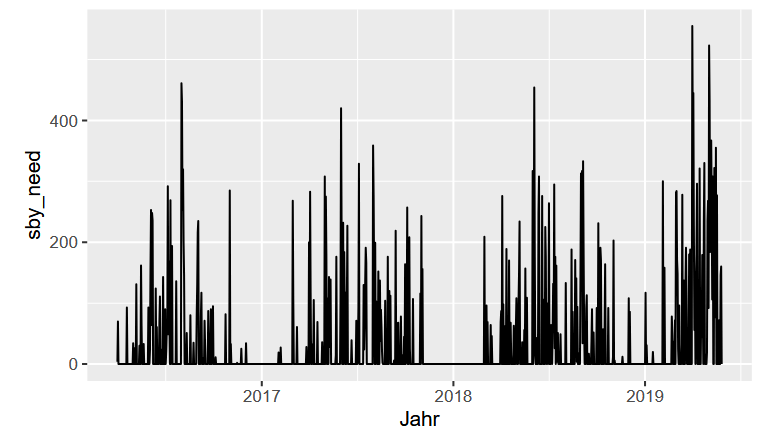
\includegraphics[width=15cm]{01_resources/timeplot_sby_need.png}\\
Quelle: Eigene Darstellung.
\label{fig:timeplot}
\end{figure}

\FloatBarrier

Die vermutete Saisonalität ist in der zeitlichen Darstellung des Bedarfs an Bereitschaftsfahrenden gut erkennbar. Augenscheinlich scheint es monatliche Spitzen in der Zielvariablen zu geben und um den Jahreswechsel ist oft nur  geringer Bedarf vorhanden. Mit dem Jahreswechsel auf 2019 ändert sich das Muster der Bedarf weist ab diesem Zeitpunkt deutlich höhere Spitzen auf. Weiters werden auch die raschen Wechsel zwischen wenig bis kein Bedarf und sehr hoher Bedarf in der Darstellung deutlich. Diese Volatilität verlangt eine überlegte Generalisierung des Modells und einen klar definierten Fokus der Vorhersage. Gemäß Aufgabenstellung ist dieser auf eine Abdeckung der Spitzenwerte ausgerichtet.

Die Korrelation zwischen der Zielvariablen und dem Merkmal der eingegangenen Notrufe wurde bereits angesprochen. Die unten angeführte Grafik macht den, nahezu linearen, Zuammenhang anschaulich.

Die Abstände im augenscheinlichen Intercept (dem Schnittpunkt mit der x-Achse) betragen zwischen den Jahren jeweils etwa 500 Notrufe. Das ist jeweils das fünffache des jährlichen Anstiegs von diensthabendem Personal. Von 2018 auf 2019 wurde das diensthabende Personal nicht erhöht, weswegen auch im Intercept der linearen Korrelation keine Veränderung erkennbar ist. Wurden weniger Anrufe als der jeweilige Intercept getätigt wurde auch kein Bereitschaftspersonal aktiviert. 

\begin{figure}[h]
\centering
\caption{Korrelation der Zielvariable zu den Notrufen}
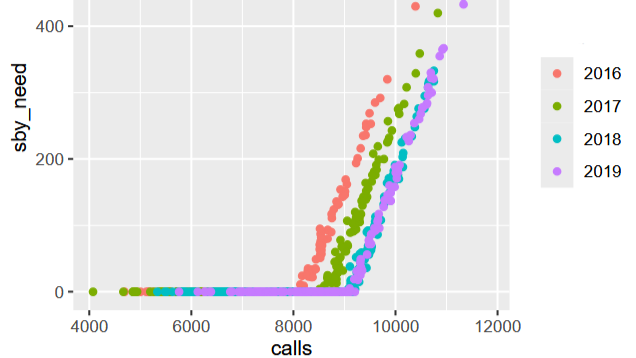
\includegraphics[width=15cm]{01_resources/call_correlation_year.png}\\
Quelle: Eigene Darstellung.
\label{fig:call_correlation_year}
\end{figure}
\FloatBarrier

Die, auf der Shannon Entropy basierende, spektrale Entropy liefert eine erste Aussage über die Verteilung und Vorhersagbarkeit von Zeitreihendaten. Im vorliegenden Datensatz wurde der beste Entropy-Wert für den gleitenden Durchschnitt der eingehenden Notrufe erzielt. Dieser wird im nachfolgenden jährlichen Saisonalitätsplot dargesellt. Die, in den Daten auftretenden, Muster sind hier gut erkennbar, genauso wie ein augenscheinlicher Aufwärtstrend über die Jahre.

\begin{figure}[h]
\centering
\caption{Verteilung der Notrufe nach Jahr}
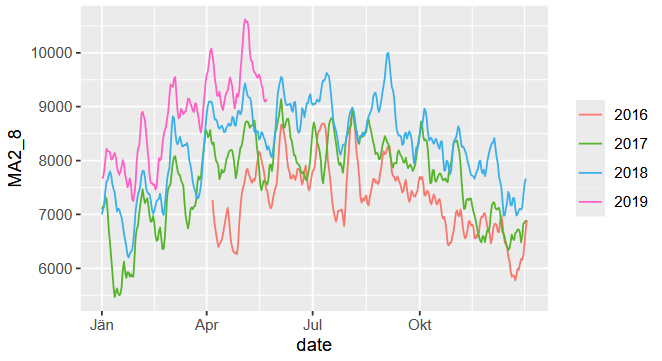
\includegraphics[width=15cm]{01_resources/calls_year.png}\\
Quelle: Eigene Darstellung.
\label{fig:callsperyear}
\end{figure}
\FloatBarrier

Die beschriebene Korrelation der Zielvariable zu den eingegangenen Notrufen (unter Berücksichtigung des diensthabenden Personals) sowie die besser modellierbare Saisonalität der eingegangenen Notrufe dienten als Grundlage für die Entwicklung fortschrittlicherer Modelle.

\section{Modeling}

Die Entwicklung der Modelle wurde mir der Programmiersprache R umgesetzt. Besonders hilfreich war hierbei das online Buch sowie das dazugehörige R Package \glqq Forecasting Principles and Practice\grqq\ \citep{hyndman_forecasting_2021}. Für die Entwicklung der Modelle wurden, wie bereits beschrieben, zwei Ansätze gewählt.  Im Vordergrund stand dabei stets die Anforderung, nie zu wenig Bereitschaftspersonal vorherzusagen. Gerade bei den vorliegenden, sehr stark und abrupt schwankenden Eingangsdaten der Zielvariablen, ist die Herausforderung, dass man zwischen Kosteneffizienz und Abdeckung der Maximalbedarfsspitzen wählen muss.  

In der explorativen Datenanalyse (Anhang \ref{app:explore}) wurde festgehalten, dass 35 Personen in Bereitschaft für Tage mit niedrigem Bedarf einen guten Durchschnittswert bilden. Die Einteilung von null Personen in Bereitschaft scheint geschäftsseitig unrealistisch, der Minimalwert wird daher für alle Modelle mit 35 Personen festgelegt.

 \subsection{Baseline Model} 

Das Baseline-Model (Anhang \ref{app:baseline}) wird direkt anhand der Saisonalität der Zielvariablen trainiert und verwendet dabei ein Lineares Model für Zeitreihen (TSLM), das auch ebenso Trends und saisonale Muster abbilden kann. Um eine ausreichende Generalisierung zu erreichen und die Vorhersage zuverlässiger zu machen, wurden die Daten mit einer, über sieben Tage, gleitenden 99\% Quantille  geglättet und anschließend zu wöchentlichen Daten aggregiert. Bei der Aggregation wurden die jeweiligen Maxima der gleitenden Quantille als Wochenwert herangezogen. Nach der Vorhersage, werden die Wochendaten wieder in Tagesdaten (gem. Anforderung) aufgetrennt, wobei die Tage einer Woche entsprechend immer denselben Wert aufweisen. Die Bedarfsspitzen werden durch dieses Model nicht korrekt vorhergesagt, die Saisonalität wird jedoch modelliert. In der Darstellung werden die Vorhersagen (blau) den Daten des Testdatensatzes (schwarz), über einen Zeitraum von zwei Monaten, gegenübergestellt. Des Weiteren werden für die Vorhersage auch die 80\%, 90\% und 99\% Konfidenzintervalle angezeigt.

\begin{figure}[h]
\centering
\caption{Vorhersage des Basline-Models}
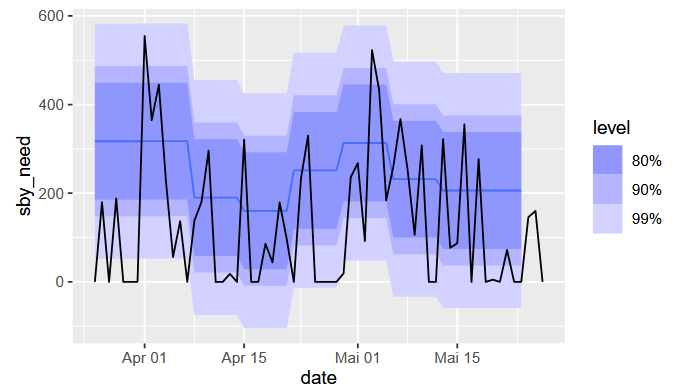
\includegraphics[width=15cm]{01_resources/baseline_prediction.png}\\
Quelle: Eigene Darstellung.
\label{fig:baseline}
\end{figure}

\FloatBarrier

Für die spätere Evaluierung wurde, als zweites Baseline-Model, auch das aktuelle Vorgehen mit einem Fixwert von 90 Bereitschaftsfahrenden mit aufgenommen.

 \subsection{Advanced Model} 

Das Advanced-Model (Anhang \ref{app:adv}) basiert auf dem Modell \glqq Seasonal and Trend decomposition using Loess\grqq\ (STL). Dieser Algorithmus wurde bereits in der explorativen Datenanalyse (Anhang \ref{app:explore}) verwendet um die saisonalen Komponeten der eingehenden Notrufe auf Basis eines gleitenden Durchschnitts zu untersuchen. Dabei werden die Daten in den Trend, verschiedene Saisonalitäten und den \glqq Remainder\grqq\ (den Rest) aufgesplittet. So können saisonale Muster in den Daten gut erkannt, analysiert und beschrieben werden. In diesem Ansatz wird jedoch nicht die Zielvariable direkt vorhergsagt sondern die, schöner modellierbare, Saisonalität der eingehenden Notrufe. Für die weitere Vorhersage des Bedarfs an Bereitschaftspersonal wird die beschriebene lineare Korrelation zwischen den eingehenden Notrufen und dem StandBy-Bedarf genutzt. Diese wurde durch ein einfaches lineares Modell abgebildet.

Die, in Punkt \ref{du} Data Understanding,  festgestellte Auswirkung der jährlichen Erhöhung des diensthabenden Personals mit einem Faktor 5 auf den Intercept der Korrelation wird im linearen Modell berücksichtigt. Bei der Anwendung des Modells muss daher die Anzahl des diensthabenden Personals als Parameter mitgegeben werden.

\[modifizierte Notrufe_t = Notrufe_t - Korrekturwert_t\ \ |\ \   Korrekturwert_t = (n\_duty_{year} - 1700) * 5\]

Der Intercept wird nach Korrektur fix auf 8150 gesetzt. Werden weniger Notrufe vorhergesagt wird durch das Model der fixierte Minimalwert von 35 Personen in Bereitschaft ausgegeben.  Die u.a. Grafik zeigt die modifizierte lineare Abhängigkeit zwischen den eingehenden Notrufen und dem StandBy Bedarf mit dem fixen Intercept bei 8150.


\begin{figure}[h]
\centering
\caption{Korrelation modifizierter Notrufdaten mit der Zielvariablen}
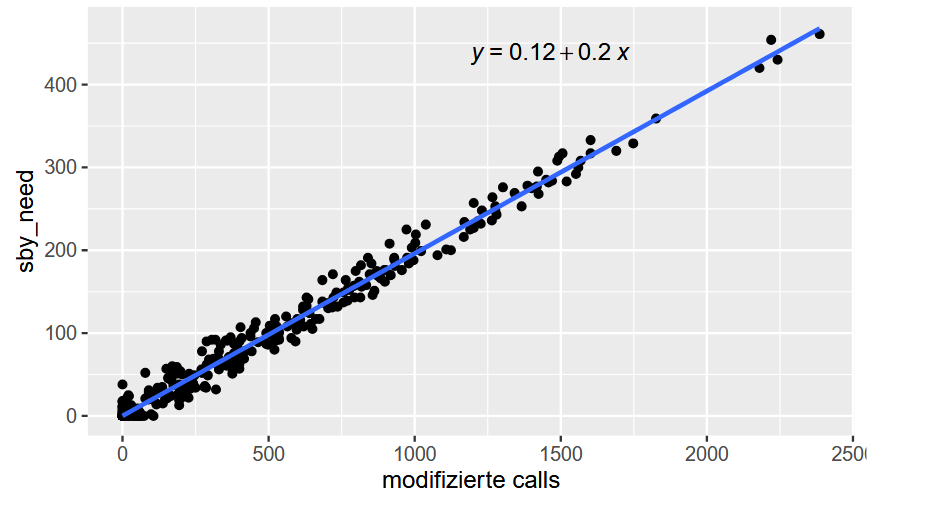
\includegraphics[width=15cm]{01_resources/reg_call_correlation_year.png}\\
Quelle: Eigene Darstellung.
\label{fig:regcall-corr-year}
\end{figure}
\FloatBarrier

Der STL Algorithmus erkennt zwar die Spitzenaufkommen in den eingehenden Notrufen, im Vergleich mit dem Testdatensatz wurden diese allerdings oft wenige Tage verschoben prognostiziert. Die, allgemein fehlende, Generalisierung der Vorhersage wird durch Anwendung eines gleitenden Maximums  auf die Prognose erreicht. 

Das Advanced Model wurde in zwei Varianten evaluiert. In den finalen Programmcode wurde allerdings nur die Version 2 aufgenommen. Der Unterschied der beiden Modelle liegt in der Fenstergröße des gleitenden Maximums und (in der Version 2) einer Reduktion des Parameters \glqq diensthabendes Personal\grqq\ um einen Wert von 100. Durch die Modifikation dieses Parameters kann die Höhe des vorhergesagten Bedarfs beeinflusst werden.

\begin{figure}[h]
\centering
\caption{Vorhersage Advanced Model V2}
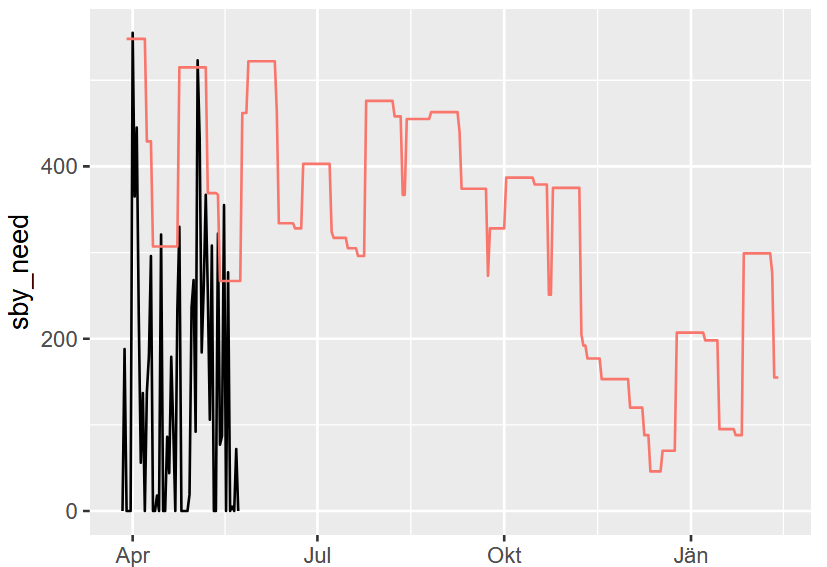
\includegraphics[width=15cm]{01_resources/adv2.png}\\
Quelle: Eigene Darstellung.
\label{fig:adv2}
\end{figure}
\FloatBarrier

Die Darstellung zeigt die Ausgabe der Vorhersage (rot) über den Zeitraum von elf Monaten. Die Werte des Testdatensatzes (schwarz) sind nur in den ersten beiden Monaten der Prognose vorhanden. Die jährliche und monatliche Saisonalität werden von dem Modell gut aufgenommen. Durch die stark ausgeprägte Generalisierung wird jedoch überwiegend eine deutlich zu hohe Anzahl an Bereitschaftspersonal vorgesehen.


 \subsection{Prophet Model} 

In der Use Case Analyse wurde der Algorithmus \glqq Facebook Prophet\grqq\ als möglicherweise passender Ansatz für die gegenständliche Machine Learning Aufgabe recherchiert. Dieser Algorithmus wurde für Zeitreihenvorhersagen entwickelt und verwendet dabei ein zusammengesetztes Modell aus Trend, Saisonalität und speziellen Ereignissen in Zeitreihen. \citep{taylor_forecasting_2017}. Der Vorteil von Facebook Prophet, oder kurz \textit{Prophet}, liegt darin, dass in einer möglichen, zukünftigen Weiterentwicklung des Modells auch Tage mit besonderen Ereignissen, wie zB Veranstaltungen und speziellen Wetterverhältnissen, mit modelliert werden können. Diese würden dann a priori in eine Vorhersage miteinbezogen und in der Prognose berücksichtigt werden.

Im Advanced-Modell wurde versucht einen Puffer für die Spitzenwerte anhand eines gleitenden Maximums über die vorhergesagten Notrufe zu erreichen. Bei Prophet erscheint die Verwendung von Konfidenzintervallen möglich. Daher wird in diesem Ansatz der Puffer durch Verwendung der 90\% Quantille als Vorhersagewert erreicht. Das Schöne hierbei ist, dass der zu verwendende Prozentsatz für die Berechnung im codierten Modell als Hyperparameter gesetzt werden kann. Wie auch im Advanced Modell V2 wird, zum Vergleich der Ergebnisse, die Höhe des diensthabenden Personals um 100 reduziert. Damit wird die Anzahl des vorhergesagten Bereitschaftspersonals etwas angehoben. 
 
\begin{figure}[h]
\centering
\caption{Vorhersage Prophet Model}
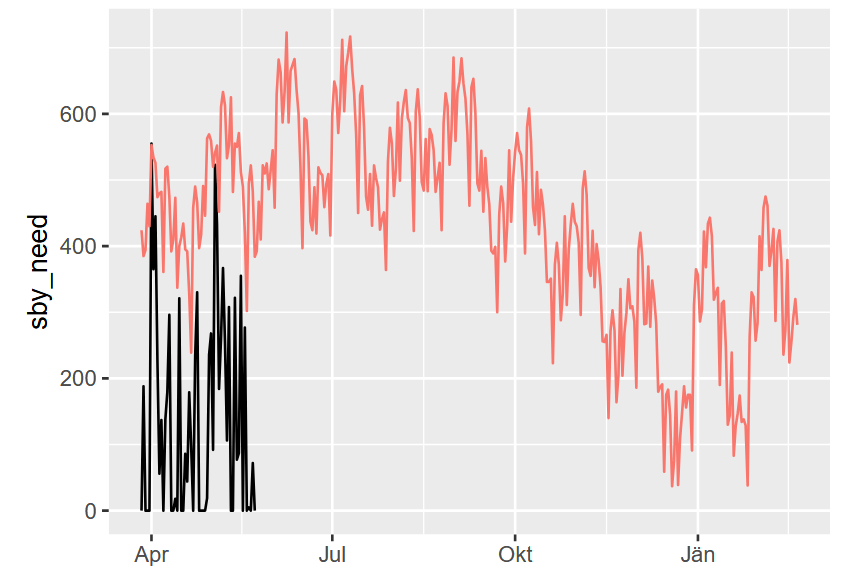
\includegraphics[width=15cm]{01_resources/prophet.png}\\
Quelle: Eigene Darstellung.
\label{fig:prophet}
\end{figure}
\FloatBarrier 

Die Darstellung zeigt wiederum die Ausgabe der Vorhersage (rot) über den Zeitraum von elf Monaten mit gleichzeitiger Anzeige der Testdaten (schwarz) für die ersten beiden Monate der Prognose. Bei Anwendung dieses Modells sind die einzelnen Komponenten der Saisonalität in der Vorhersage zu erkennen. Man sieht sowohl den jährlichen Verlauf mit einem Abfall des Bedarfs bis zum Jahreswechsel, als auch ein augenscheinlich relativ fixes Muster in den Monatsdaten. Der Grad der Flexibilität in den saisonalen Mustern kann in Prophet durch Hyperparameter gesteuert werden. In diesem Bereich bietet Prophet auch die meisten Möglichkeiten das Modell noch feiner zu \glqq tunen\grqq\ . Das Machine Learning Framework \textit{Caret} \citep{kuhn_caret_2019} bietet Unterstützung im Finetuning durch ein automatisieretes \glqq Durchtesten\grqq\ mehrerer Kombinationen an Hyperparametern. Das war in dem, hier verwendeten, Package \textit{fpp3} \citep{hyndman_forecasting_2021} nicht möglich, dafür ist dieses speziell für die Arbeit mit Zeitreihen entwickelt. In einer Weiterentwicklung des gegebenen Anwendungsfalles wäre ein Hyperparameter-Finetuning für den Prophet-Ansatz jedenfalls zielführend. 

Dank Verwendung der 90\% Quantille für die Prognose, wird auch bei diesem Modell überwiegend eine zu hohe Anzahl an Bereitschaftspersonal vorgesehen. Die Höhe der Vorhersage ist, wie auch beim Advanced Model, über gesetzte Parameter beeinflussbar und sollte mit den Entscheidungsträgern noch diskutiert werden.

\newpage 

\subsection{Modellresultate} 

\begin{table}[h]
\centering
\caption{Vergleich der ML-Modelle}
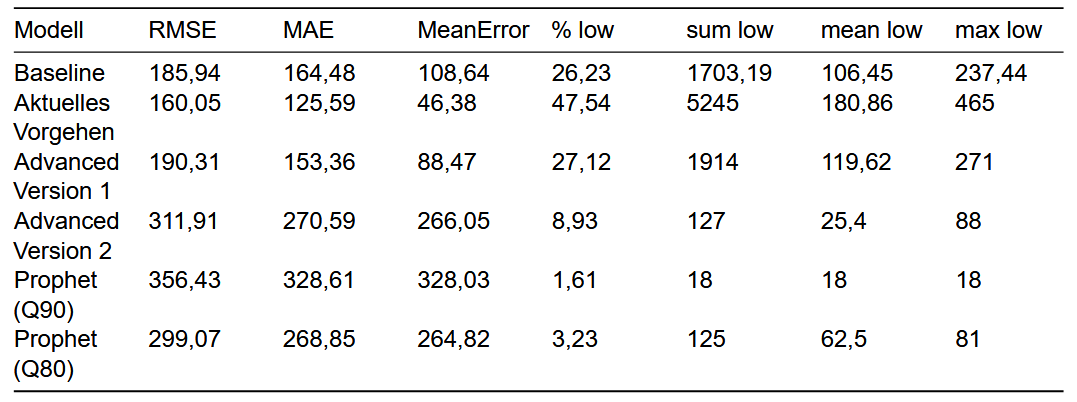
\includegraphics[width=15cm]{01\_resources/modellvergleich.png}\\
Quelle: Eigene Darstellung.
\label{tab:modeleval}
\end{table}
\FloatBarrier 

Die angeführte Tabelle zeigt einen Vergleich der beschriebenen Modelle (inklusive des aktuellen Vorgehens) anhand unterschiedlicher Messwerte. Diese sind folgendermaßen zu interpretieren:

\begin{itemize}
 \itemsep-8pt
 \item \textbf{RMSE}: Gängiger Messwert. Berechnet die Wurzel der mittleren quadrierten Abweichung
 \item \textbf{MAE}: Gängiger Messwert. Berechnet die durchschnittliche absolute Abweichung
 \item \textbf{MeanError}: Die durchschnittliche Abweichung. Positive Werte deuten auf eine durchschnittliche Überschätzung durch das Modell hin
 \item \textbf{\% low}: Prozentanteil der Vorhersagen, wo das Modell zu niedrig geschätzt hat
 \item \textbf{sum low}: Die Summe zu niedrig geschätzten Personals, gleichzeitig Personal, das zusätzlich hätte aktiviert werden müssen.
 \item \textbf{mean low}: Der Durchschnitt jener Schätzungen, die unter dem Bedarf lagen. 
 \item \textbf{max low}: Die maximale Abweichung jener Schätzungen, die unter dem Bedarf lagen.
 \end{itemize}


Die, in der obigen Tabelle, dargestellten Messwerte beziehen sich auf eine Gütebewertung der Modelle in einem Testzeitraum von zwei Monaten. Hierbei wird ersichtlich, dass beim bisherigen Vorgehen etwa bei der Hälfte der Tage zu wenig Bereitschaftspersonal vorgesehen wurde. In den zwei Monaten Testzeitraum hätten in Summe 5245 zusätzliche Bereitschaftsfahrer:innen aktiviert werden müssen. Hinsichtlich einer durchschnittlichen Abweichung (RMSE, MAE oder MeanError) schneidet das aktuelle Vorgehen jedoch am Besten ab. Eine erste Verbesserung in Bezug auf Unterschätzungen des Bedarfs an Bereitschaftspersonal zeigen das Baseline Modell und das Advanced Modell in der Version 1. Die beiden Modelle liefern ähnliche Messwerte und schaffen es Unterschätzungen auf ein Viertel der Vorhersagen zu senken, wohingegen RMSE und MAE noch mit dem aktuellen Vorgehen vergleichbar bleiben. Das Advanced Modell in Version 2, sowie zwei Varianten des Prophet Modells (einmal mit 80\% Konfidenzintervall und einmal mit 90\% Konfidenzintervall) steigen bei RMSE und MAE deutlich in die Höhe, was sich, im Gegenzug, in einer ebenso deutlichen Verringerung der Fälle von Unterschätzung widerspiegelt. 

Auf welches Modell, die Entscheidung schlussendlich fällt ist abzuwägen und wird mit den Entscheidungsträgern diskutiert werden müssen. Durch \glqq Finetuning\grqq\ von Hyperparametern ist gegebenenfalls noch eine Verbesserung einzelner Modelle zu erreichen. Derzeit sind die Modelle \glqq Baseline\grqq\ , \glqq Advanced V2\grqq\ und \glqq Prophet Q90\grqq\ ausprogrammiert.

Für alle Modelle ist die Rechendauer als sehr positiv zu bewerten. Die Zeiten für Training und Vorhersage betrugen, in der Entwicklung, beim Baseline Modell in Summe 0,28 Sekunden, bei den Advanced Modellen in Summe 0,97 Sekunden und den Prophet Modellen in Summe 13,60 Sekunden. Für die Entwicklung wurde ein Notebook vom Typ Dell Latitude 5490, Intel i7 vPro (8th Gerneration) mit 16 Gb RAM (aus dem Jahr 2018) verwendet. Für eine Umsetzung der modellbasierten Vohersage im Bereitschaftsdienst ist daher nicht mit großen Anschaffungskosten hinsichtlich Hardwarekapazitäten zu rechnen.

\subsubsection{Fehleranalyse} 
Die Schwachsellen der vorgestellten Modelle, liegen, wie bereits im Vergleich erkennbar, in der Unfähigkeit sowohl niedrigen als auch hohen Bedarf korrekt vorherzusagen. Hier wird eine Entscheidung getroffen werden müssen, worauf der Fokus liegen soll. Eine korrekte Vorhersage von Tagen mit niedrigem Bedarf spart Bereitschaftskosten, wohingegen der Einsatz von zu wenig Bereitschaftsfahrenden möglicherweise einen Reputationsschaden nach sich ziehen kann. 
An dieser Stelle wäre es hilfreich mit den Entscheidungsträgern gemeinsam eine Use Case spezifische Kostenfunktion für die Bewertung der Modelle zu entwerfen. Diese kann dann die tatsächlichen Kosten der Vorhersage ermitteln. 

Weiters ist es für Modelle des maschinellen Lernens schwierig, allgemeine Änderungen im Muster der Daten (Datendrift) abzubilden. Beim vorliegenden Datensatz ist mit dem Jahreswechsel 2018/2019 eine solche Änderung erkennbar. Diese fällt in einen Zeitraum, der bereits die Testdaten für die Gütebewertung der Modelle beinhalten und daher nicht für das Training herangezogen werden sollte. Das Sammeln weiterer Trainingsdaten, die das Aufkommen nach 2019 beschreiben könnte die Modellgüte maßgeblich verbessern. Bei den vorgestellten Modellen, ist der Prophet Algorithmus auch in der Lage, vorgegebene \textit{Changepoints} für Änderungen im Trend zu berücksichtigen. So könnten zB auch maßgebliche Trendwenden wie COVID-19 modelliert werden.

\section{Solution Architecture}

Die Implementierung des Vorhersagemodells in die tägliche Arbeit der Planungsstelle könnte dermaßen erfolgen, dass die Mitarbeitenden weiterhin täglich die Betriebsmetriken (wie auch im vorliegenden Datensatz), über ein Formular festhalten. Dieses kann, wie in der unteren Grafik dargestellt auch in Form einer Web-Applikation bereitgestellt werden.

Am 10. Tag jedes Monats wird über eine weitere Seite der Web-Applikation das Training und die Vorhersage für einen angegebenen Zeitraum (zB zwei Monate) angestoßen und die Mitarbeiter:innen erhalten die prognostizierten Werte als Liste und grafisch ausgegeben.

\begin{landscape}
\centering
\captionof{figure}{mögliches Dateneingabe-GUI} 
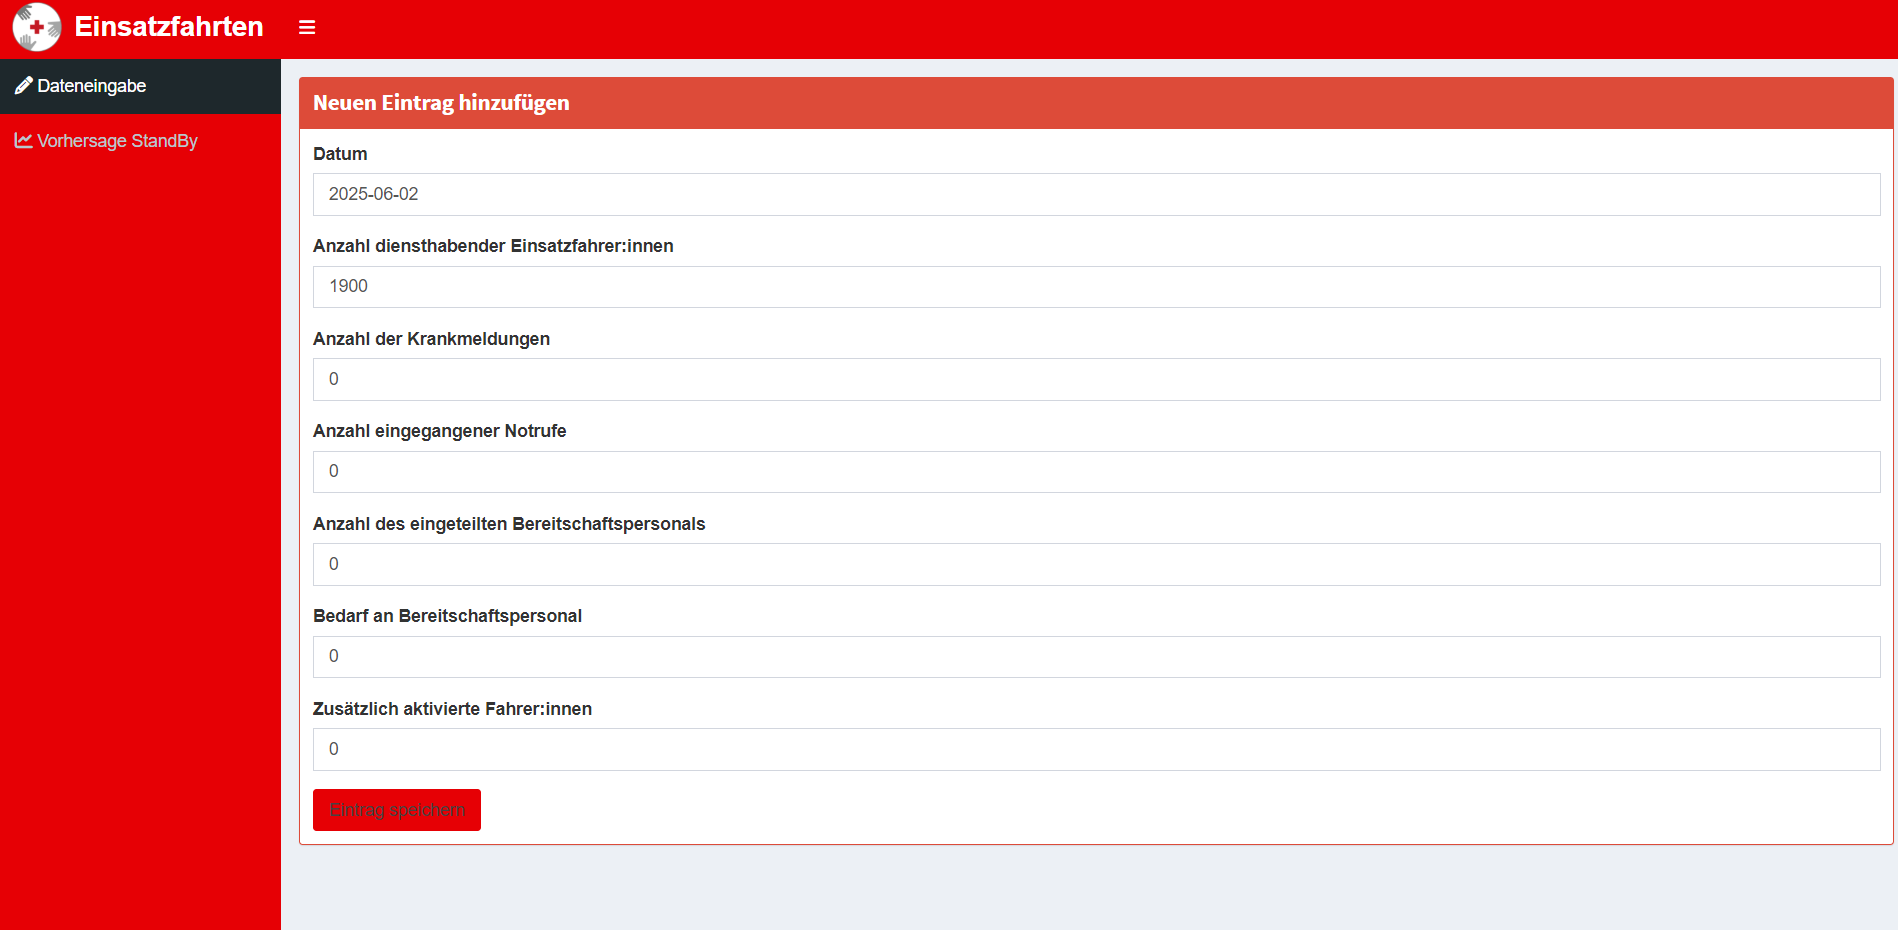
\includegraphics[width=22cm]{01_resources/dataentry.png}\\
Quelle: Eigene Darstellung.
\label{fig:dataentry}
\end{landscape}
\FloatBarrier 
  
\begin{landscape}
\centering
\captionof{figure}{mögliches Datenausgabe-GUI} 
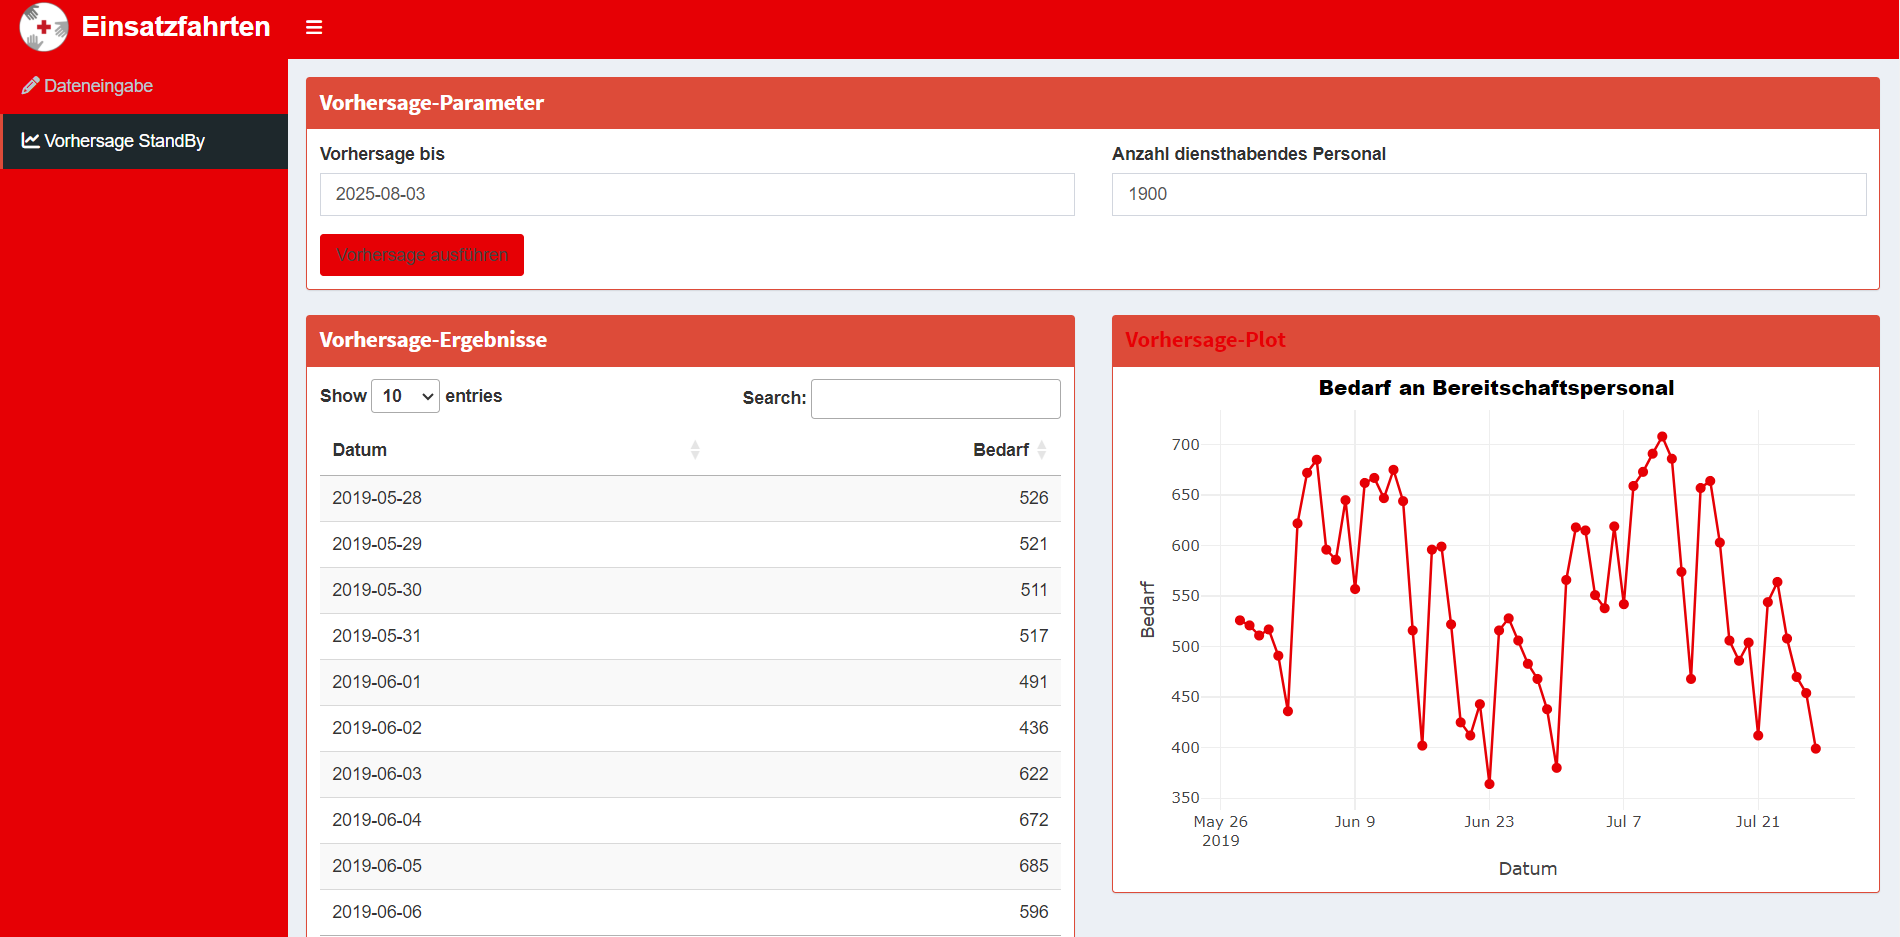
\includegraphics[width=22cm]{01_resources/dataforecast.png}\\
Quelle: Eigene Darstellung.
\label{fig:forecast}
\end{landscape}
\FloatBarrier
 
Die Planungsstelle hat nun noch weitere fünf Tage Zeit, diese Werte 

 \begin{enumerate}
  \itemsep-8pt
   \item	auf Plausibilität zu prüfen und eigene Erfahrung mit einfließen zu lassen. Prognostizierte Werte dürfen vom Personal der Planungsstelle abgeändert werden, das Bedarf allerdings klaren Regeln und einer hinreichenden Dokumentation, wie in Punkt Customer Acceptance (\ref{ca}) noch erläutert wird.
   \item mit Namen von Bereitschaftspersonal zu hinterlegen und so einen Bereitschaftsdienstplan zu erstellen.
 \end{enumerate}
 
Das Format der Ausgabe durch die Web-Applikation kann noch den Wünschen Planungspersonals angepasst werden. Zur nachvollziehbaren Modellbewertung sollte die Prognose nicht veränderbar (read-only) gespeichert werden. Abänderungen durch die Planungsstelle müssen gesondert dokumentiert und abgelegt werden.

Die derzeit im Repository verfügbare Web-Applikation bildet die Grundfunktionalität des beschriebenen Ablaufes dar. Dennoch sind hier noch einige Weiterentwicklungen und Verbesserungen für einen Betrieb vorzusehen. Hierzu gehören zum Beispiel die Änderung und Bearbeitung bereits angelegter \glqq Betriebsmetriken\grqq\ , oder auch die angesprochene Speicherung und Dokumentation von Prognosemodifikationen durch die Planungsstelle. Weiters wäre es sinnvoll, zusätzlich zu Training und Vorhersage, auch einen Trainings- und Testlauf, mit allen verfügbaren Modellen, anhand der gespeicherten historischen Daten durchführen zu können (zB durch Aktivieren einer Check-Box) und die Modellbewertungen analog zu Tabelle (\ref{tab:modeleval}), oder mit eigener Kostenfunktion, anzeigen lassen zu können. So kann in periodischen Abständen überprüft werden ob die Vorhersagealgorithmen in einem zuverlässigen Rahmen arbeiten, oder ob sich die Güte einzlner Modelle (zB aufgrund eines Datendrifts) verschlechtert.

Die Auswahl des anzuwendenden Vorhersagemodells wurde in der Web-Applikation bewusst weggelassen. Die Mitarbeitenden der Planungsstelle sollen sich nicht damit beschäftigen müssen, welches Modell, wie funktioniert und auch nicht begründen, warum sie welches Modell gewählt haben. Es wäre jedoch keine Schwierigkeit ein solches Feature in die Applikation zu implementieren, da beim Training derzeit das Prophet Modell standardmäßig beim Funktionsaufruf als Parameter mitgegeben wird, die Funktion aber so gestaltet ist, dass durch Veränderung dieses Parameters jedes implementierte Modell gewählt werden kann. 

Für die Implementierung neuer Modelle ist demnach auch einfach nur der Code für das Modell, analog zur Struktur und Namenskonvention bestehender Modelle im Ordner \textit{04a\_model\_standby\\03\_deployment} abzulegen und in der Applikation mit dem Parameter des Modellnamens aufzurufen. Sollten neue Modelle weitere zusätzliche Hyperparameter benötigen sind diese jedoch applikationsweit zu ergänzen.

Die, diesem Projekt vorangegangene, Use Case Analyse sieht für die geschäftszentrierte Messung des Erfolgs ein Monitoring der Vorhersagemodelle anhand von zwei Key Result Indikatoren (KRI) vor. Diese sind zwar nicht ausschließlich von der Arbeit der Vorhersage abhängig, spiegeln jedoch die Messung des, durch Implementierung der Modelle, gewünschten Effekts wider. Die beiden Werte werden in der Use Case Analyse \citep{grunsky_rettungsdienst_2024} wie folgt beschrieben:

\begin{itemize}
 \itemsep-8pt
 \item Eine statistisch aufbereitete Messung der „time-to-target“ , also der Zeit vom Anruf bis zum Eintreffen am Einsatzort bzw. der „no-shows“ , das sind Notrufe, die nicht bedient werden konnten. Natürlich hängen diese Werte von viel mehr Faktoren ab, als den verfügbaren Bereitschaftsfahrer:innen. Die Vermeidung von Totalausfällen (no-shows) aufgrund mangelnden Bereitschaftspersonals wird aber eine wesentliche Ziffer für den Erfolg des Modells darstellen.
 \item  Die mittleren Personalkosten pro Notruf sollten mit einer akkuraten Planung der Bereitschaftsfahrenden eigentlich abnehmen. Wenn man den o.a. Wert als K.O.-Kriterium für die Modellbewertung erachtet, so sagt dieser Wert (im Vergleich mit Vorangegangenen) aus, wie präzise das Modell arbeitet.
\end{itemize}

In der Use Case Analyse wurde davon ausgegangen, dass ein Vorhersagemodell sowohl niedrigen als auch erhöhten Bedarf korrekt vorhersagen würde. Die Modellentwicklung hat hier bis dato etwas anderes ergeben. Aus aktueller Sicht scheinen die beiden angeführten KRIs  für das Monitoring des Modells im gegenständlichen Anwendungsfall trotzdem Gültigkeit zu besitzen und könnten noch zusätzlich in die Applikation mit aufgenommen werden. In diesem Fall müsste nur noch die Frage geklärt werden, wer für die Dokumentation der erforderlichen Metriken verantwortlich ist.


\section{Benefits}
\label{ca}
Sowohl im Rahmen der Use Case Analyse \citep{grunsky_rettungsdienst_2024} als auch der Projektplanung \citep{grunsky_rettungsdienst_2025} wurden die Stakeholder des Projektes beleuchtet.  

Den \textbf{Bereitschaftsfahrenden} kommt der eine erfolgreiche Umsetzung des Vorhersagemodells zugute. Durch eine ausreichende Abdeckung werden kurzfristige Anrufe, ob man nicht evtl. doch Dienst versehen kann vermieden und die persönliche Freizeit dadurch planbarer. 

Für den \textbf{Rettungsdienst} bedeutet eine erfolgreiche Umsetzung möglicherweise eine Kostenersparnis, wenn geringerer Bedarf korrekt vorhergesagt würde, aber in jedem Fall die Vermeidung eines Reputationsschadens aufgrund mangelden Bereitschaftspersonals.

Die \textbf{Planungsstelle} sieht sich im täglichen Betrieb sogar mit zusätzlichem Aufwand und größerer Verantwortung konfrontiert. Dank des Vorhersagemodells wird nun nicht mehr, wie bisher, ein vorgegebener Tages-Fixwert angenommen sondern der von einem Sysem ermittelte wahrscheinliche Bedarf an Bereitschaftspersonal. Die Mitarbeiter:innen der Planungsstelle können diesen Wert nun übernehmen oder dokumentiert und begründet Abändern. In jedem Fall übernehmen Sie, anders als bisher, die Verantwortung für die Höhe des eingeteilten Bereitschaftspersonals. Das Präsidium hat mit dem Auftrag für dieses Modell bereits angeordnet, dass eine zu geringe Besetzung des Bereitschaftsdienstes unbedingt zu vermeiden ist. Diese neue Verantwortung könnte dazu führen, dass die Mitarbeitenden der Planungsstelle den Einsatz des Systems ablehnen, da sie dadurch nur verlieren können. Dieses Risiko wurde in der Projektplanung auch als eines der Hauptrisiken identifiziert.

Eine klar geregelte Vorgehensweise, um den Mitarbeiter:innen der Planungsstelle auch in ungewissen Fällen Sicherheit zu geben, ist zwingend notwendig. Auch die Einbeziehung der Nutzer in das Projekt, gleich von Beginn an, kann dabei helfen, die Identifikation dieser mit dem \glqq selbst mitgestalteten\grqq\ System zu erhöhen und ihnen die Angst vor der Benutzung oder deren Konsequenzen zu nehmen (oder diese zumindest frühzeitig zu erkennen). 

\begin{figure}[h]
\centering
\caption{Risiko Nutzerakzeptanz}
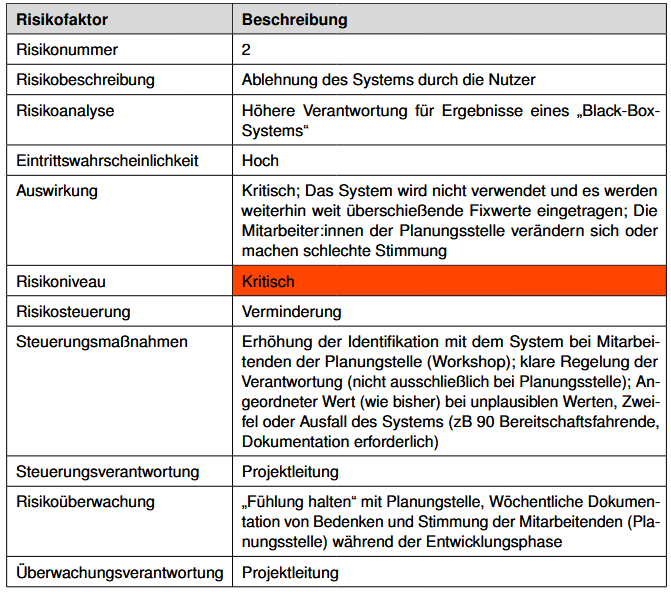
\includegraphics[width=15cm]{01_resources/risk2.png}\\
Quelle: \cite{grunsky_rettungsdienst_2025}
\label{fig:risk2}
\end{figure}
\FloatBarrier 


\section{Learnings}
\label{learned}

Durch die Umsetzung dieses Projektes von der Use Case Analyse über die Projektplanung bis hin zu einer ersten Entwicklung konnte ein tieferes Verständnis für das Zusammenspiel bestehender Werkzeuge, die Bedeutung von Schnittstellen und Struktur in der Arbeit mit diesen Werkzeugen aber auch die Unzulänglichkeiten mit der Prozesse und Frameworks teils spezifiziert sind, erlangt werden. 

Speziell auf die Entwicklung der Modelle bezogen, erweiterte die Arbeit mit Machine Learning Frameworks in R wie \textit{caret} \citep{kuhn_caret_2019} und \textit{fpp3} \citep{hyndman_forecasting_2021}, aber auch mit Werkzeugen wie Quarto \citep{posit_quarto_2025} das eigene Repertoire der Entwicklung und half dabei eine eigene Vorlage und Arbeitsweise für zukünftige Projekte anzulegen.

Nächste Schritte in diesem Projekt sollten 

\begin{itemize}
 \itemsep-8pt
 \item eine Diskussion mit dem Präsidium über die Definition einer fallspezifischen Kostenfunktion,
 \item das Finetuning von Hyperparametern, sowie
 \item die Umsetzung eines modell- und geschäftszentrierten Monitorings der Vorhersagemodelle 
\end{itemize}

enthalten.









\chapter{Zusammenfassung}



% ---- Bibliography ----
%
% BibTeX users should specify bibliography style 
% References will then be sorted and formatted in the correct style.
%
\bibliographystyle{iubh}
\raggedright % Ausrichtung linksbündig
\bibliography{biblio_neu}

\listoffigures %List of figures
\listoftables %list of tables
%% Abbreviations list

%\renewcommand\refname{Abbreviations} 
\chapter{Abkürzungsverzeichnis}
% The abbreviations list should contain all abbreviations that are not common-knowledge.
\begin{acronym}[RLHF] % the longest abbreviation here (for layout)
    \setlength {\itemsep}{-\parsep} % geringerer Zeilenabstand    	
    \acro{AI}{Artificial Intelligence}
    \acro{KI}{Künstliche Intelligenz}
    \acro{GPT}{Generative Pre-trained Transformer Model}
    \acro{PPO}{Proximal Policy Optimization}
    \acro{NLP}{Natural Language Processing}
    \acro{RLHF}{Reinforcement Learning from Human Feedback}
    \acro{FAQ} {Frequently Asked Questions}
\end{acronym}

% Acronyms should be made hyperreffed the first time they appear in text with
% \ac{GPT}  


\appendix 
\chapter{Annexes}

\section{MachineLearning-Canvas}
\label{onepager}
\begin{center}
\includegraphics[scale=1, angle = 90, origin=c]{pics/mlcanvas.png} 
\end{center}



%\chapter{Glossary (optional)}

%\chapter*{Eidesstattliche Erklärung}

\begin{figure}[t!]
    \raggedleft
    
\includegraphics[scale=0.3]{pics/logo.pdf}
\end{figure}

\thispagestyle{empty} %Seitenzahl weglassen

I hereby certify...


\vspace{1,5 cm} 
\begin{tabular}{p{7cm}p{.5cm}l}
\dotfill \\ 
Place, date
\end{tabular}% 
\hfill 
\begin{tabular}{p{7cm}p{.5cm}l}
\dotfill \\ 
Signature
\end{tabular}% 

\end{document}
